\section{Distribution of Number of Trackjets in the large-$R$ jet}
\label{app:ntrkjet}

This is a check on the number of trackjet distribution in the Sideband (Figure ~\ref{fig:boosted-ntrk-Sideband}), Control (Figure ~\ref{fig:boosted-ntrk-Control}) and Signal regions (Figure ~\ref{fig:boosted-ntrk-Signal}). Overall, the agreement is great.


\begin{figure*}[htbp!]
\begin{center}
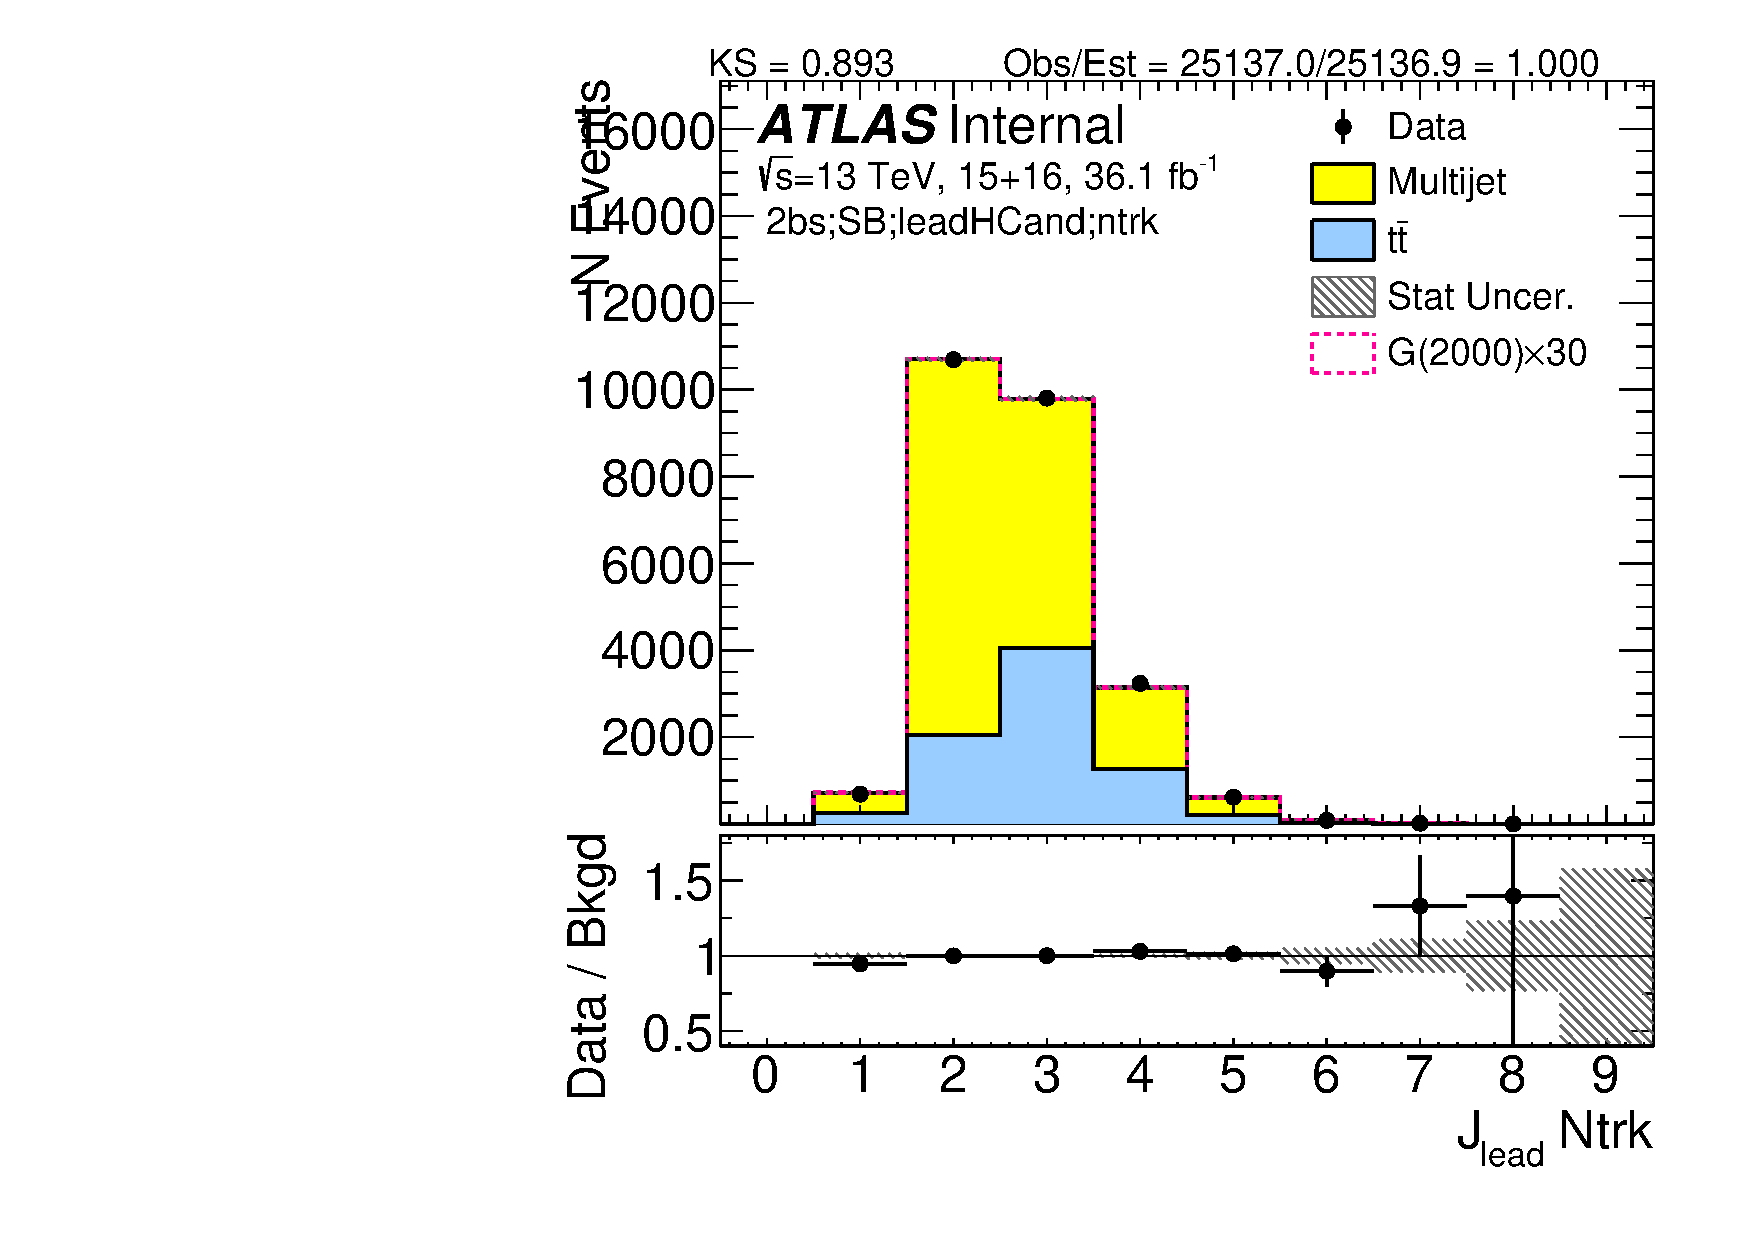
\includegraphics[width=0.45\textwidth,angle=-90]{figures/boosted/Sideband/b77_TwoTag_split_Sideband_leadHCand_ntrk.pdf}
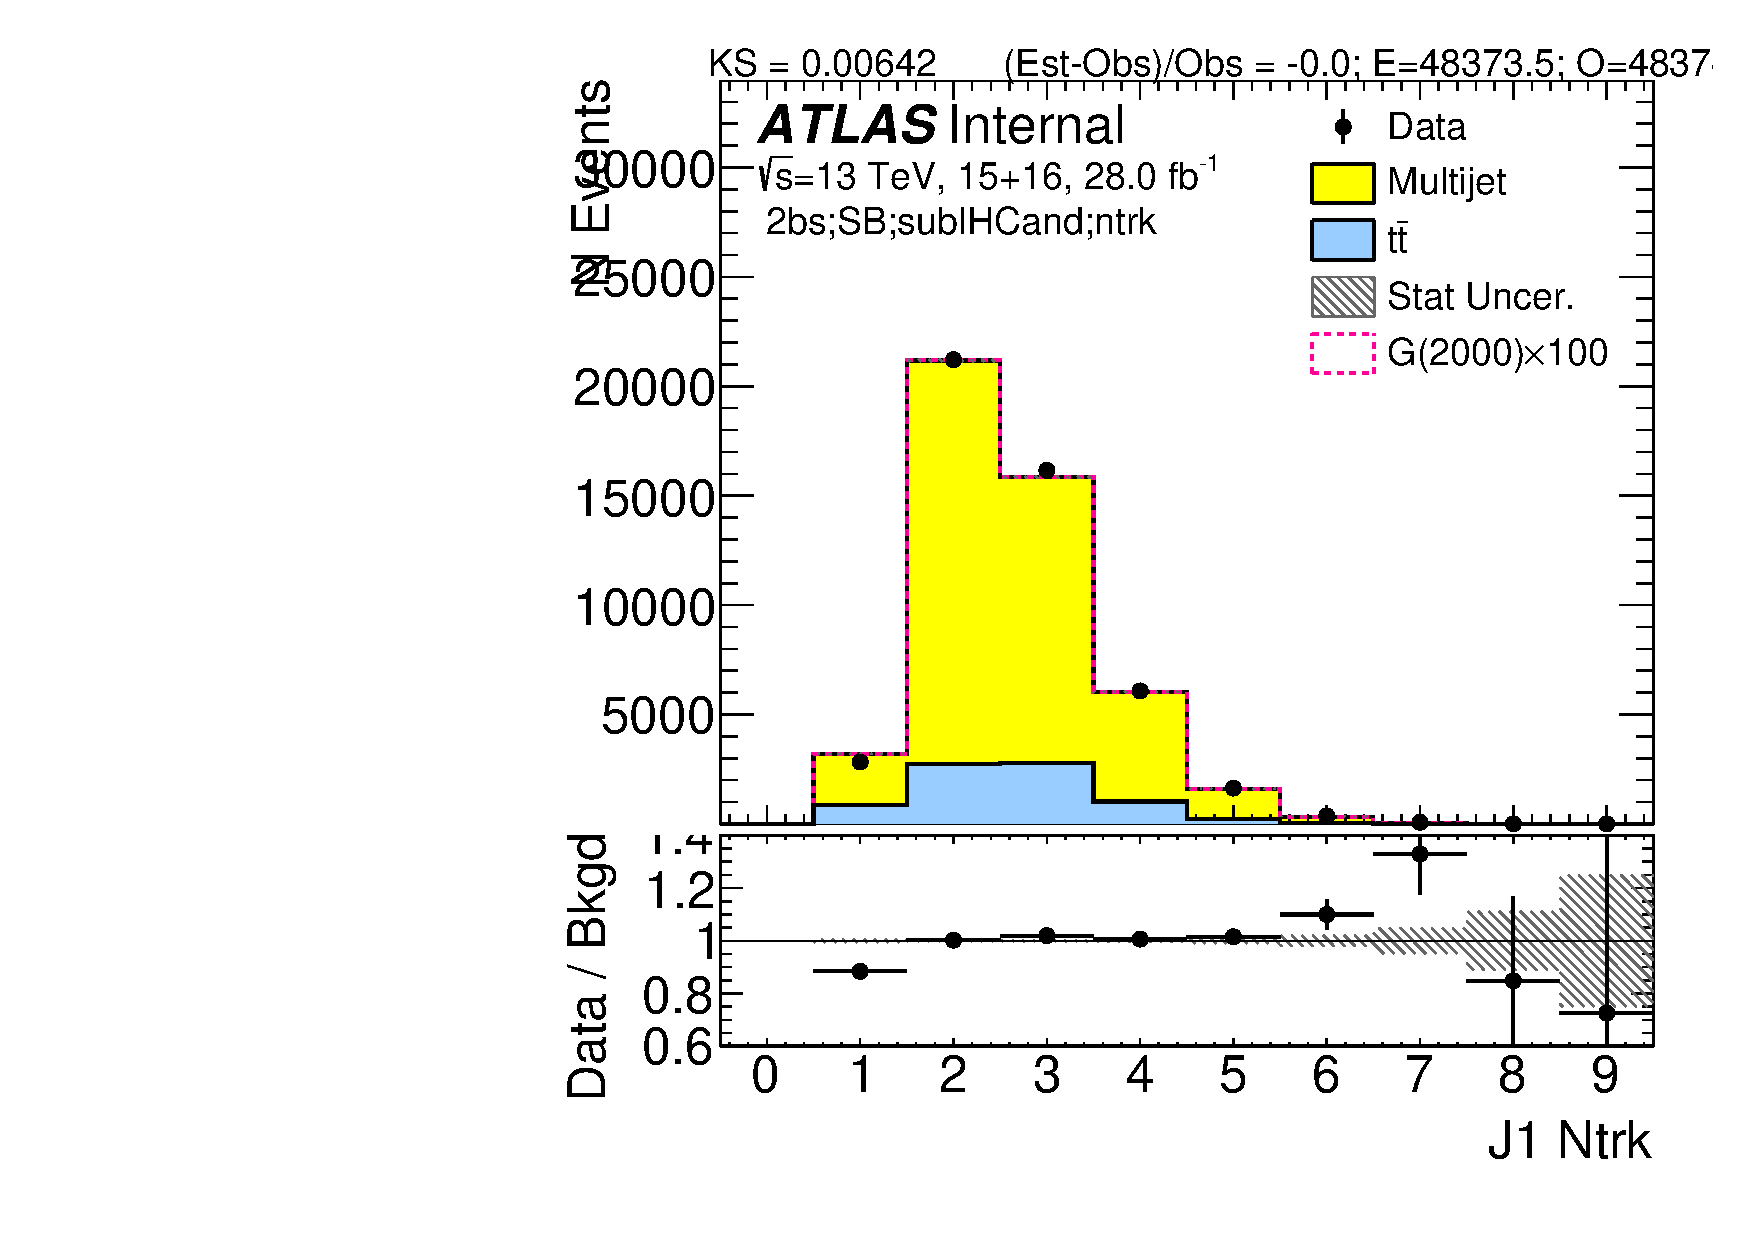
\includegraphics[width=0.45\textwidth,angle=-90]{figures/boosted/Sideband/b77_TwoTag_split_Sideband_sublHCand_ntrk.pdf}\\
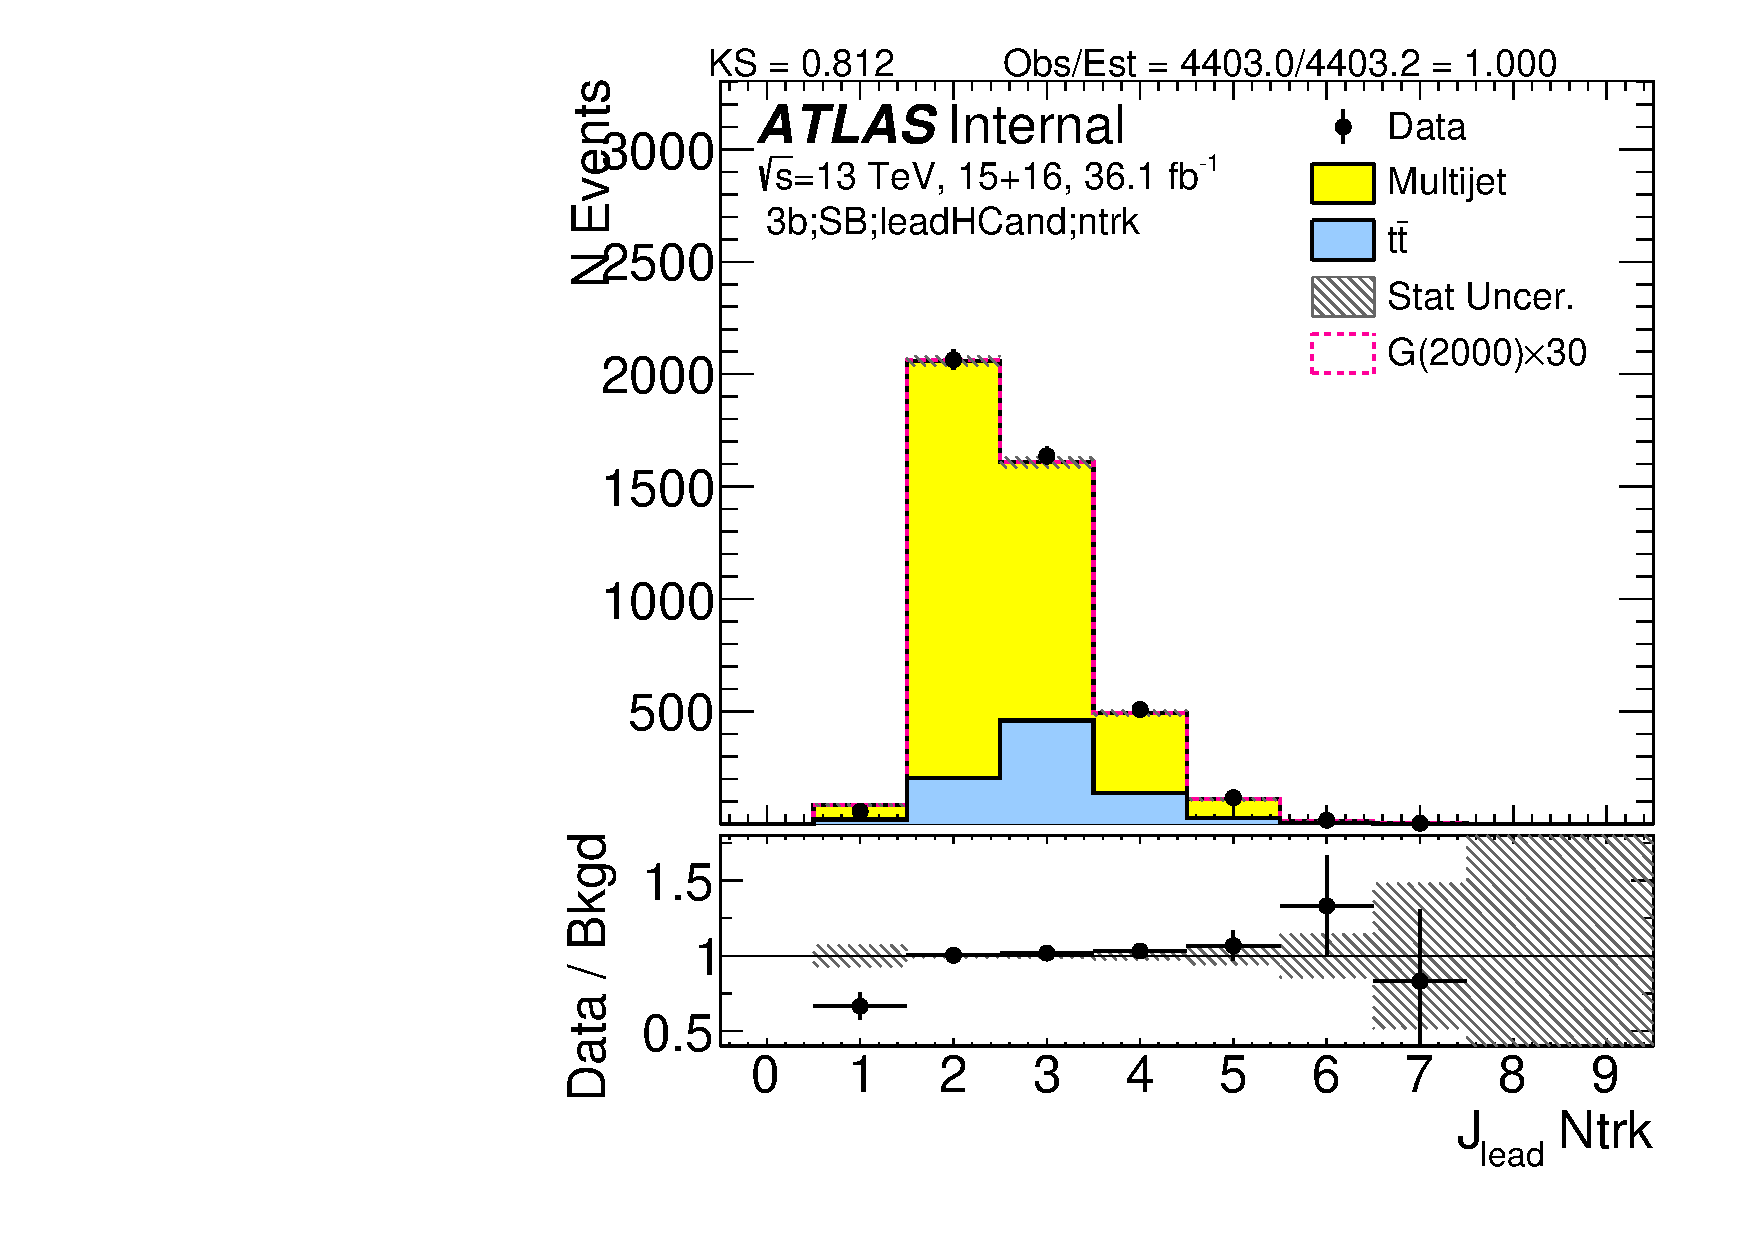
\includegraphics[width=0.45\textwidth,angle=-90]{figures/boosted/Sideband/b77_ThreeTag_Sideband_leadHCand_ntrk.pdf}
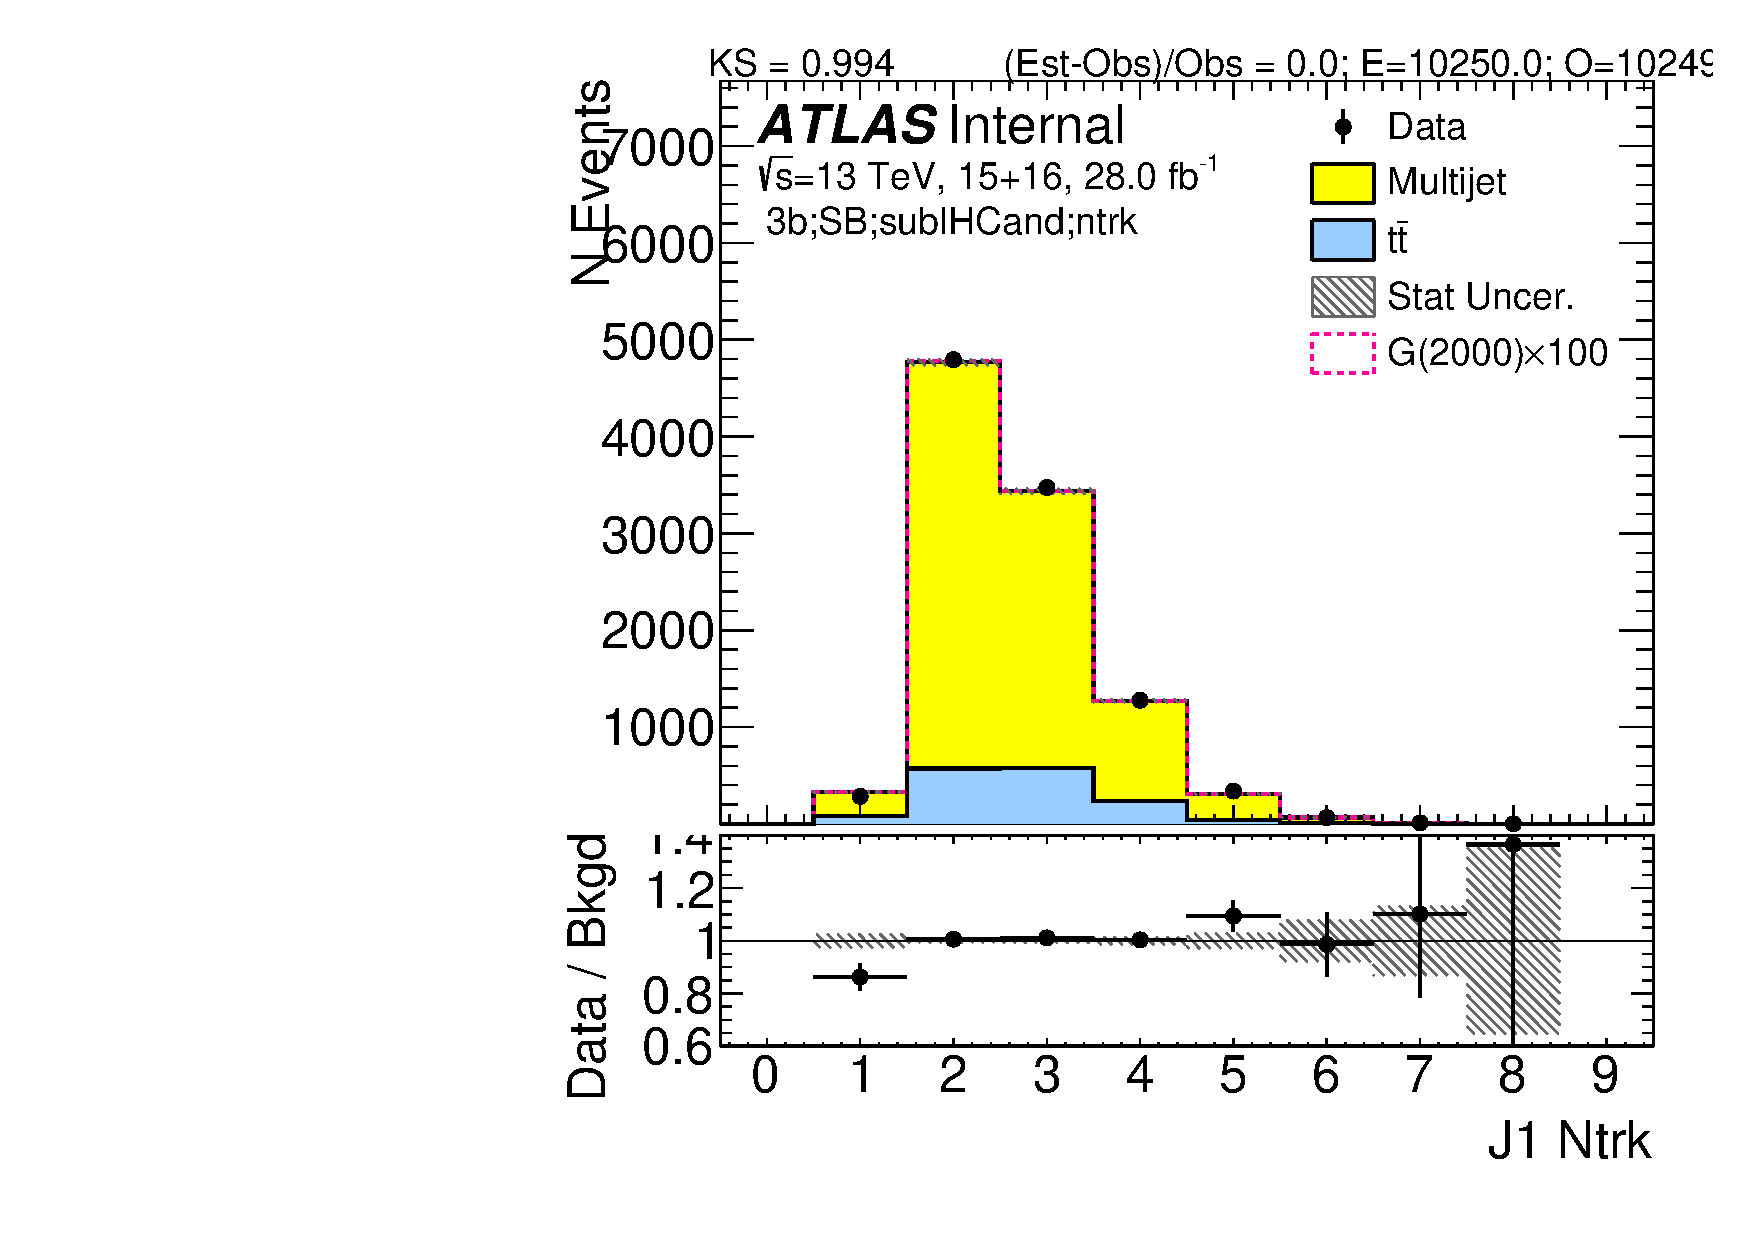
\includegraphics[width=0.45\textwidth,angle=-90]{figures/boosted/Sideband/b77_ThreeTag_Sideband_sublHCand_ntrk.pdf}\\
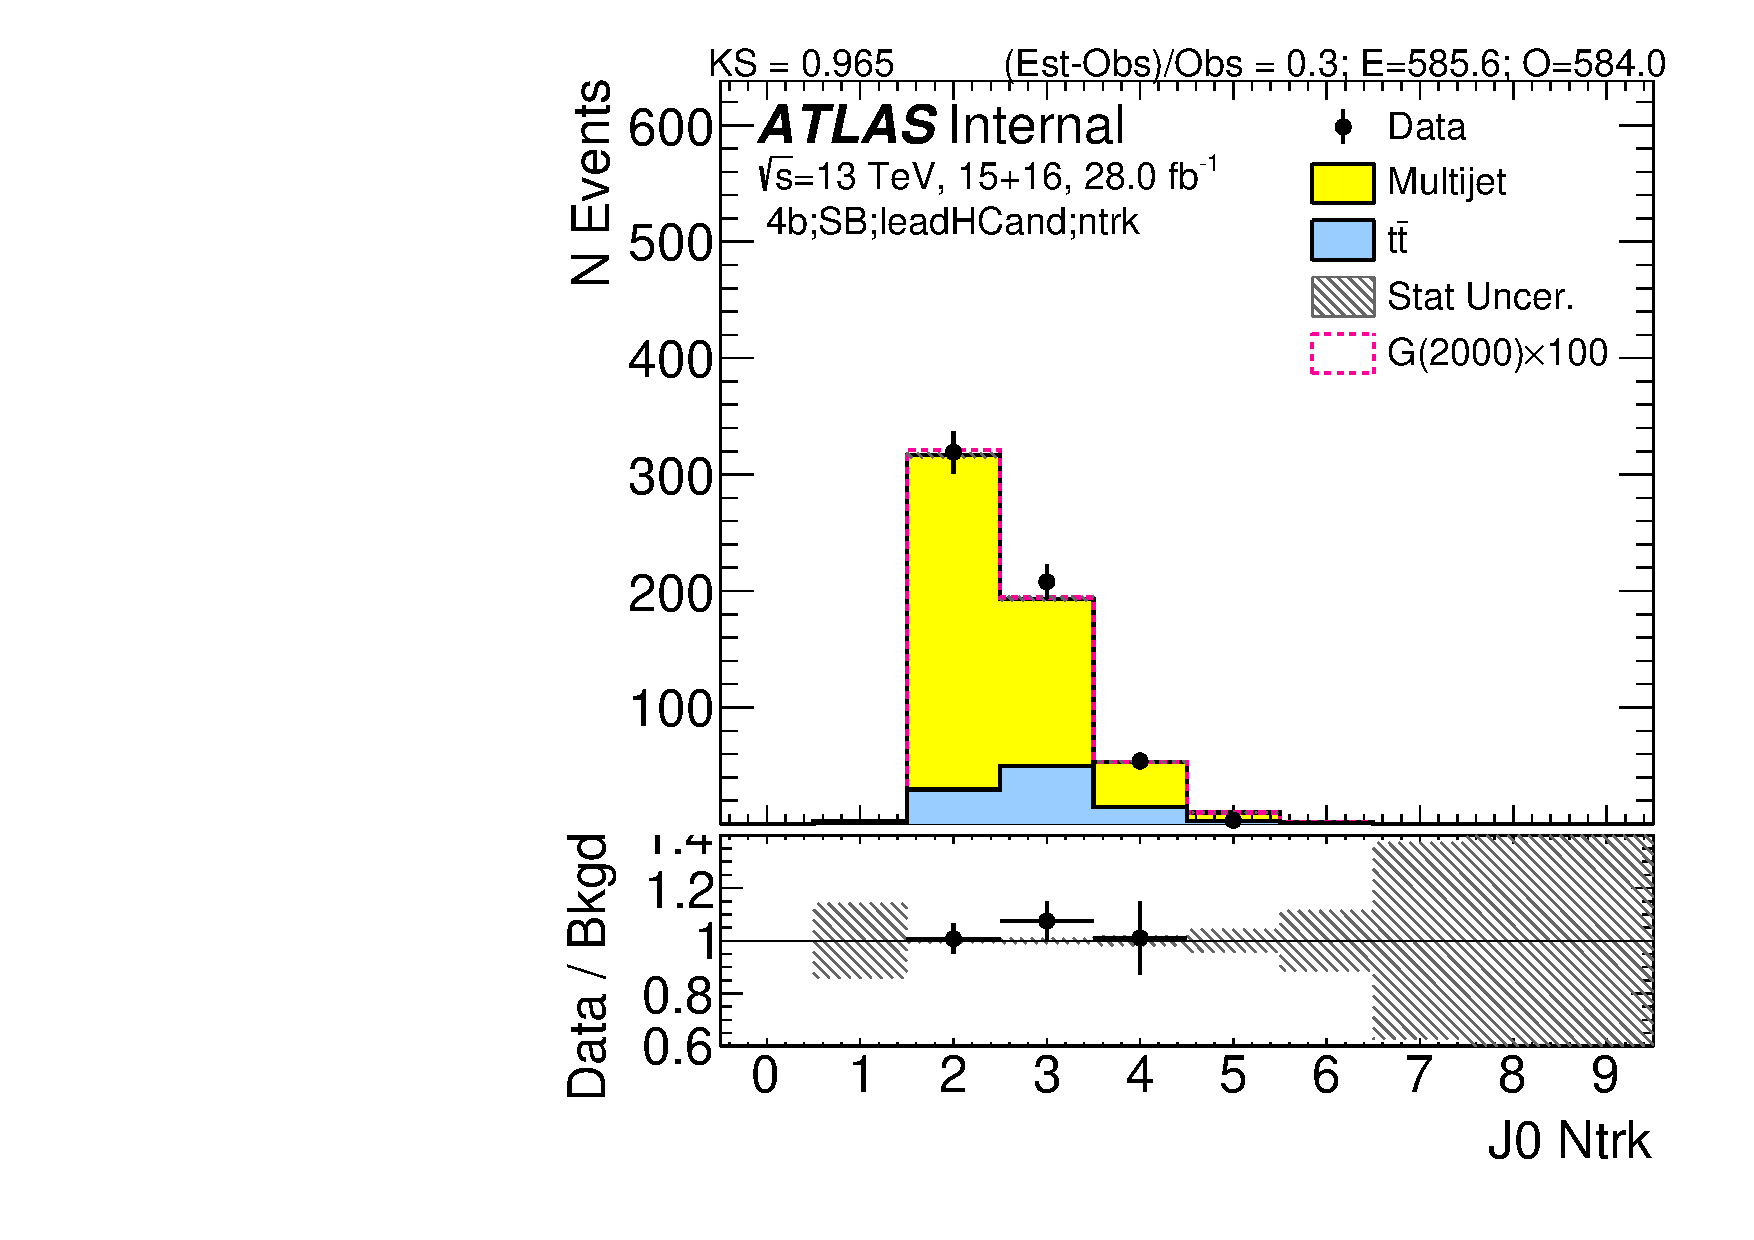
\includegraphics[width=0.45\textwidth,angle=-90]{figures/boosted/Sideband/b77_FourTag_Sideband_leadHCand_ntrk.pdf}
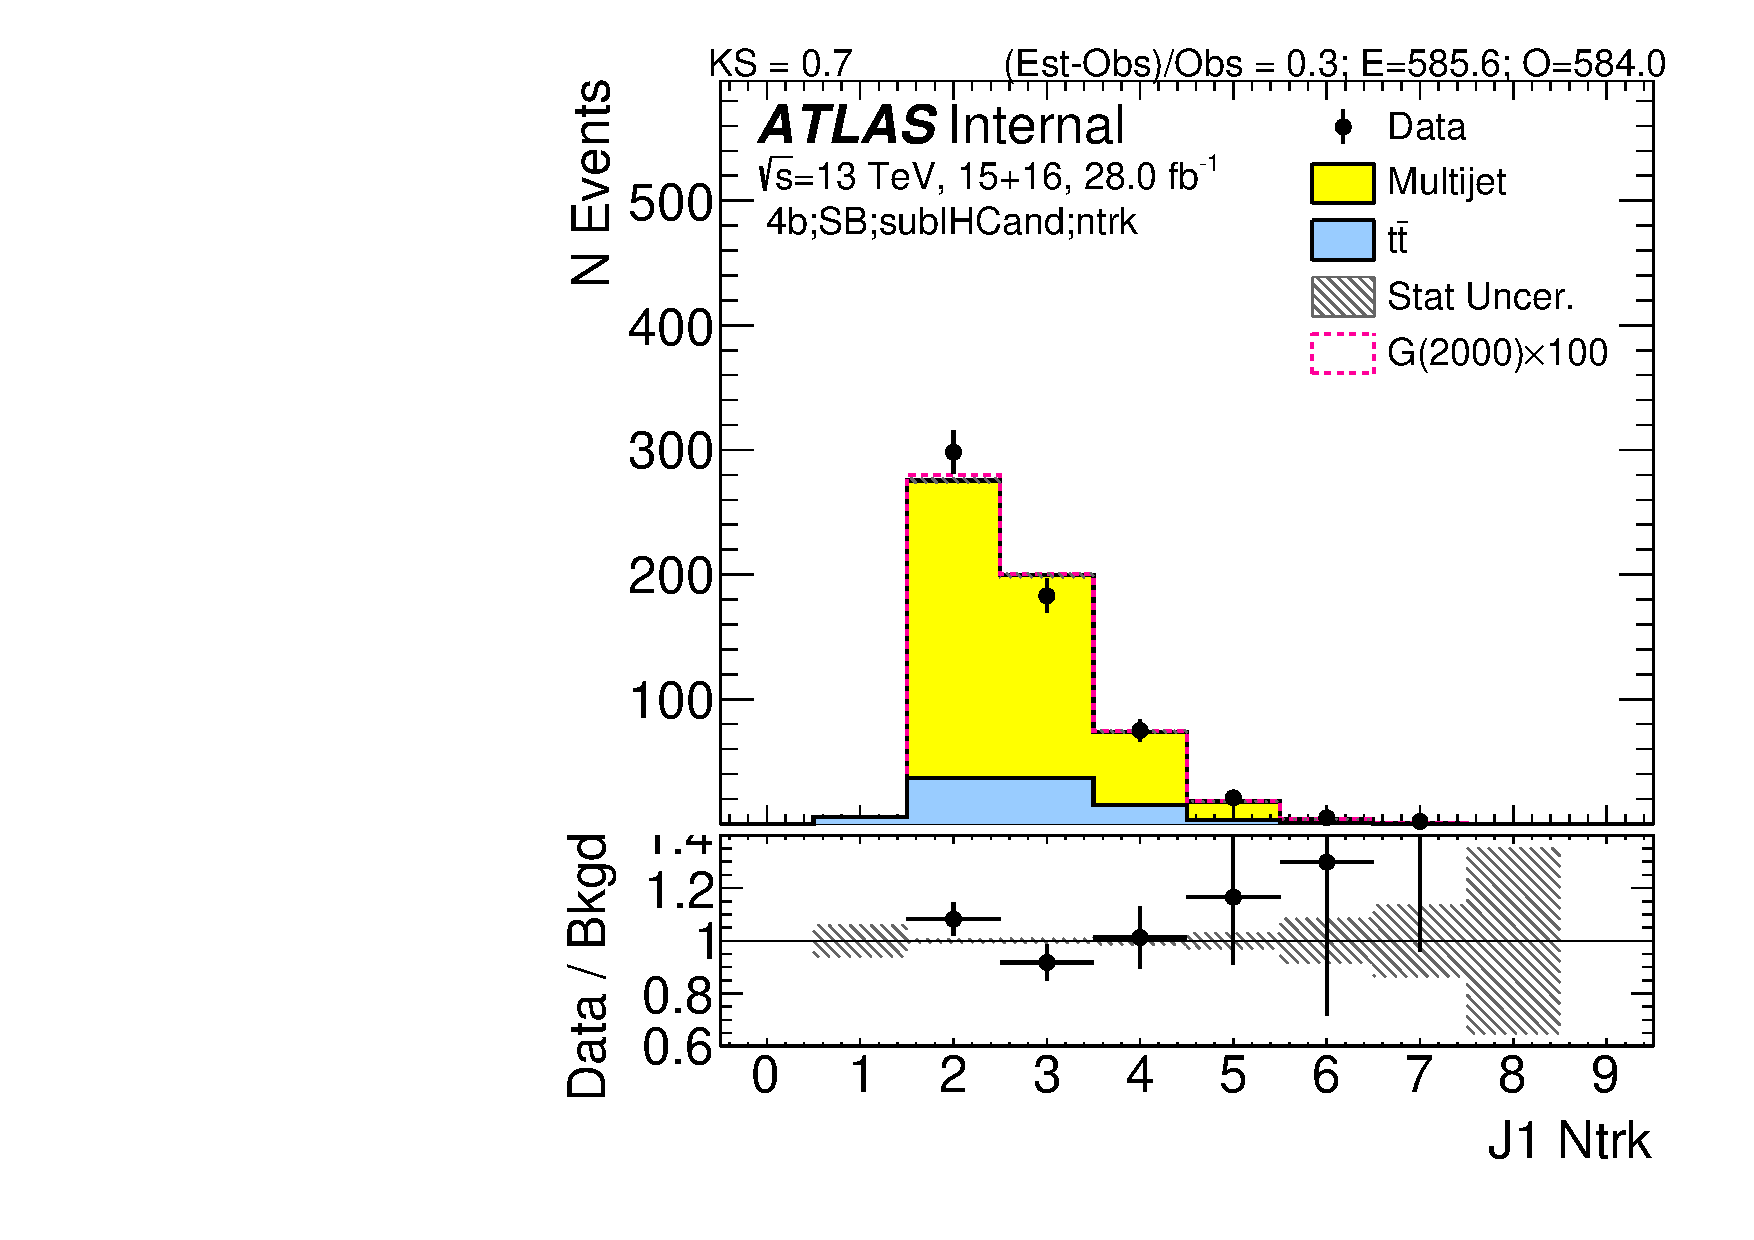
\includegraphics[width=0.45\textwidth,angle=-90]{figures/boosted/Sideband/b77_FourTag_Sideband_sublHCand_ntrk.pdf}
  \caption{Number of trackjets in the leading (left) and subleading (right) large-$R$ jet in the Sideband region for 2bs (top), 3b (middle) and 4b (bottom).}
  \label{fig:boosted-ntrk-Sideband}
\end{center}
\end{figure*}

\begin{figure*}[htbp!]
\begin{center}
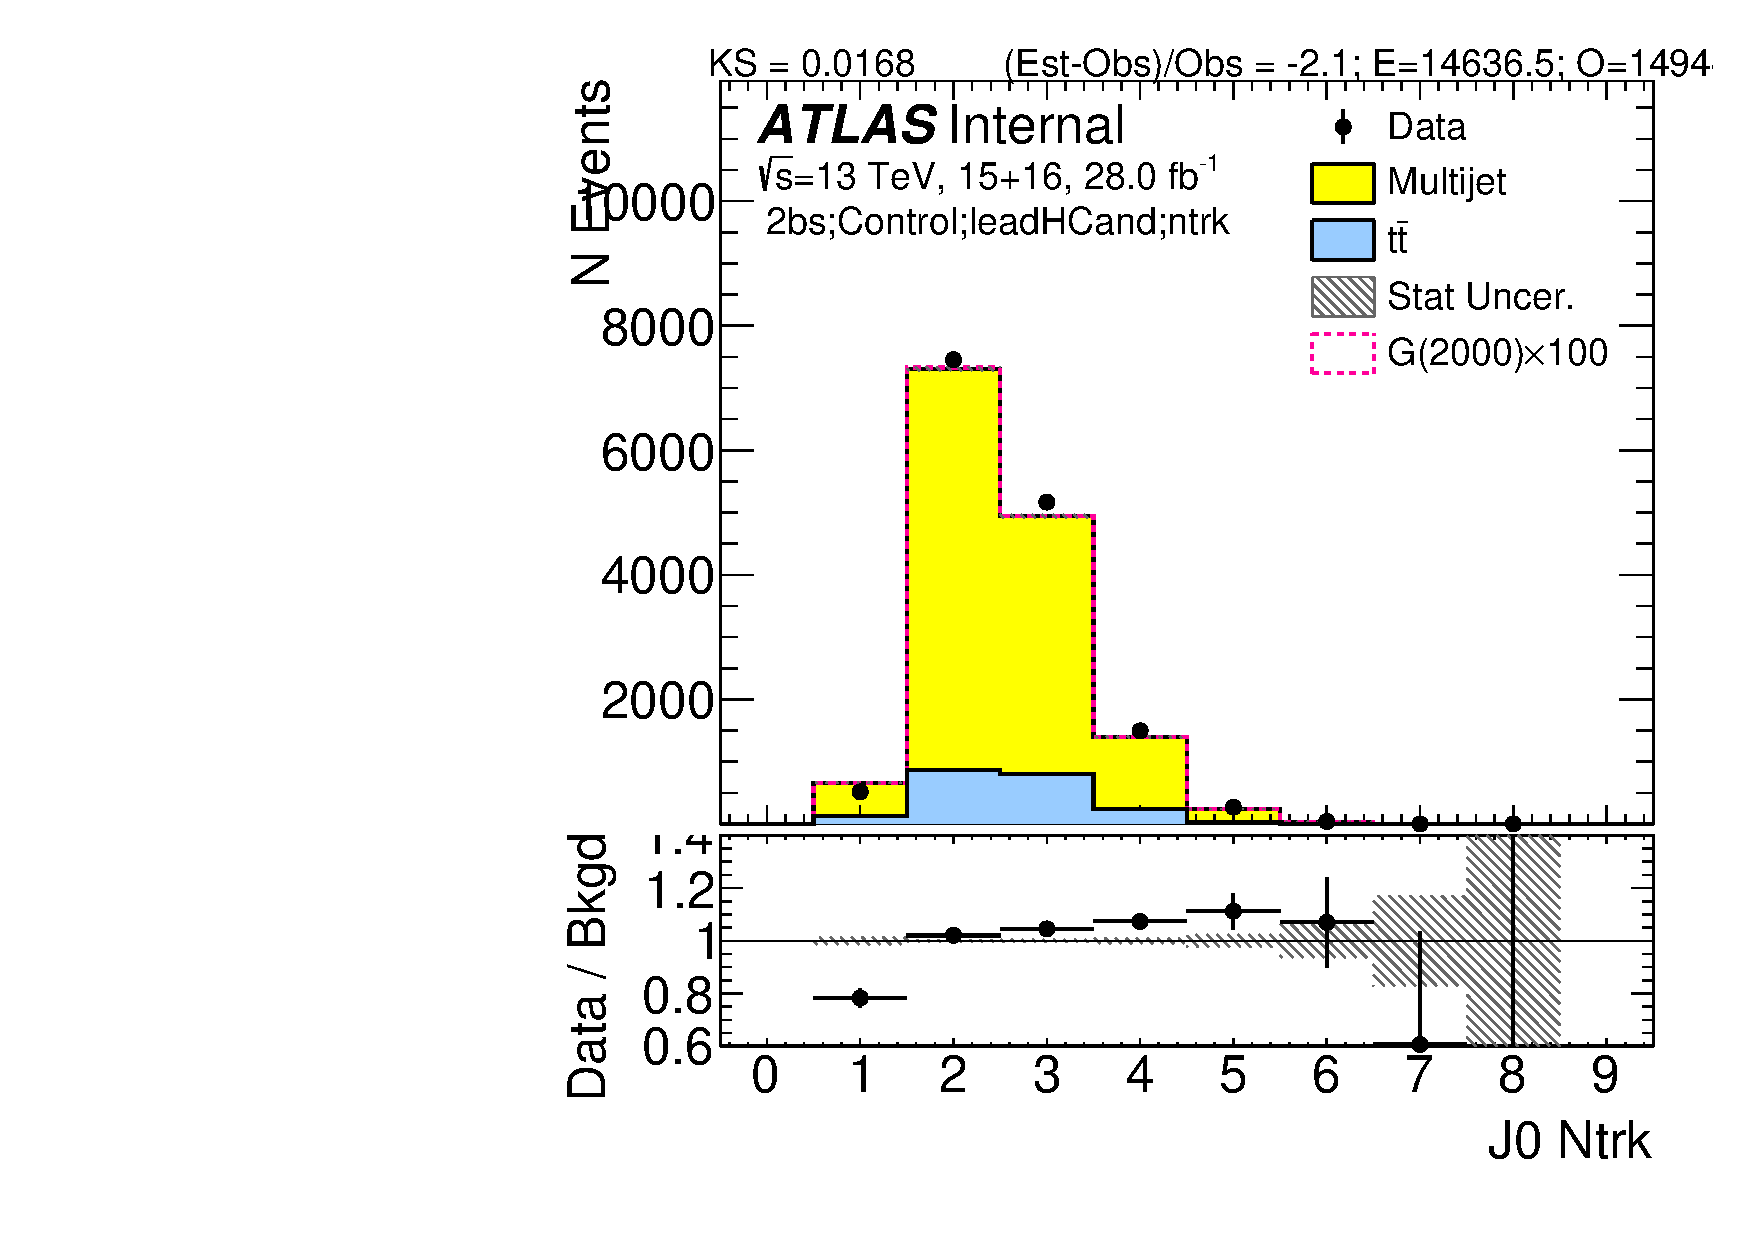
\includegraphics[width=0.45\textwidth,angle=-90]{figures/boosted/Control/b77_TwoTag_split_Control_leadHCand_ntrk.pdf}
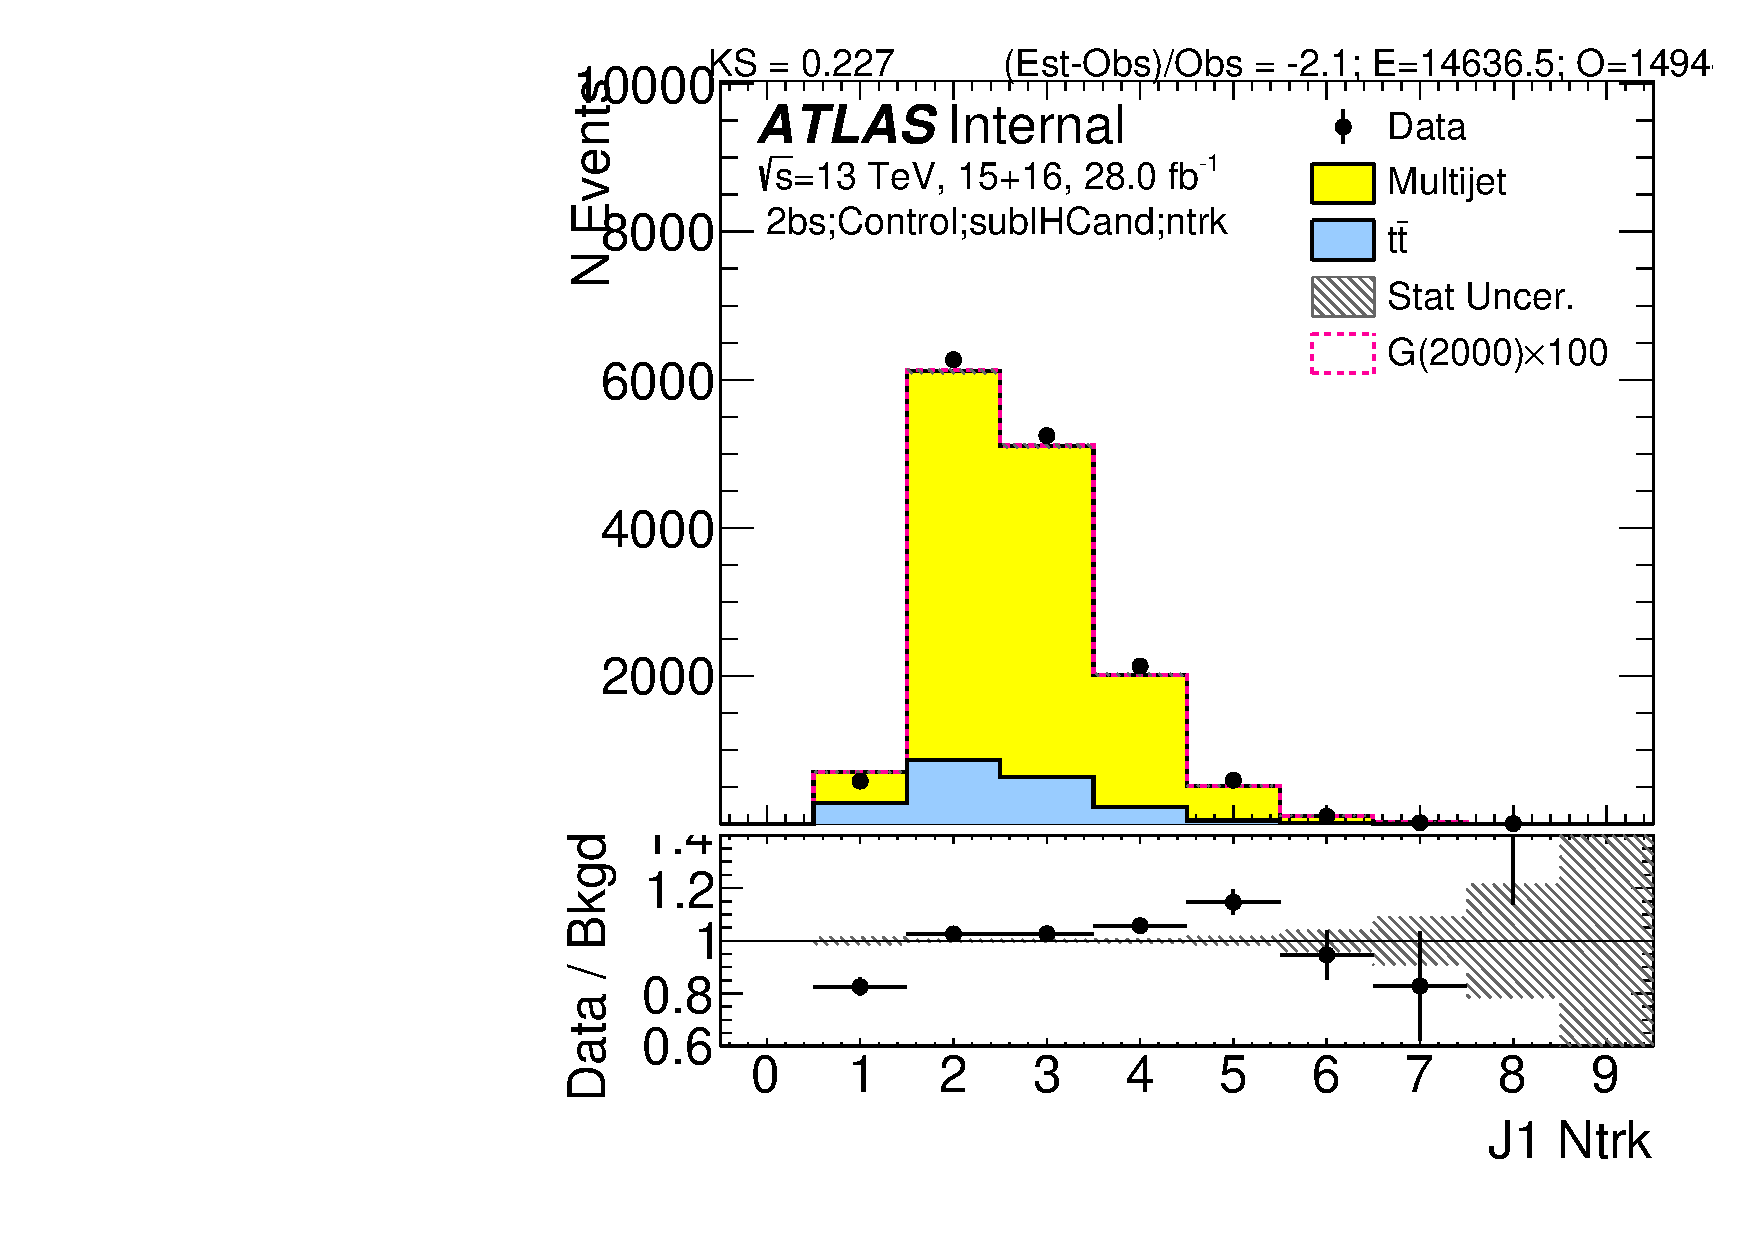
\includegraphics[width=0.45\textwidth,angle=-90]{figures/boosted/Control/b77_TwoTag_split_Control_sublHCand_ntrk.pdf}\\
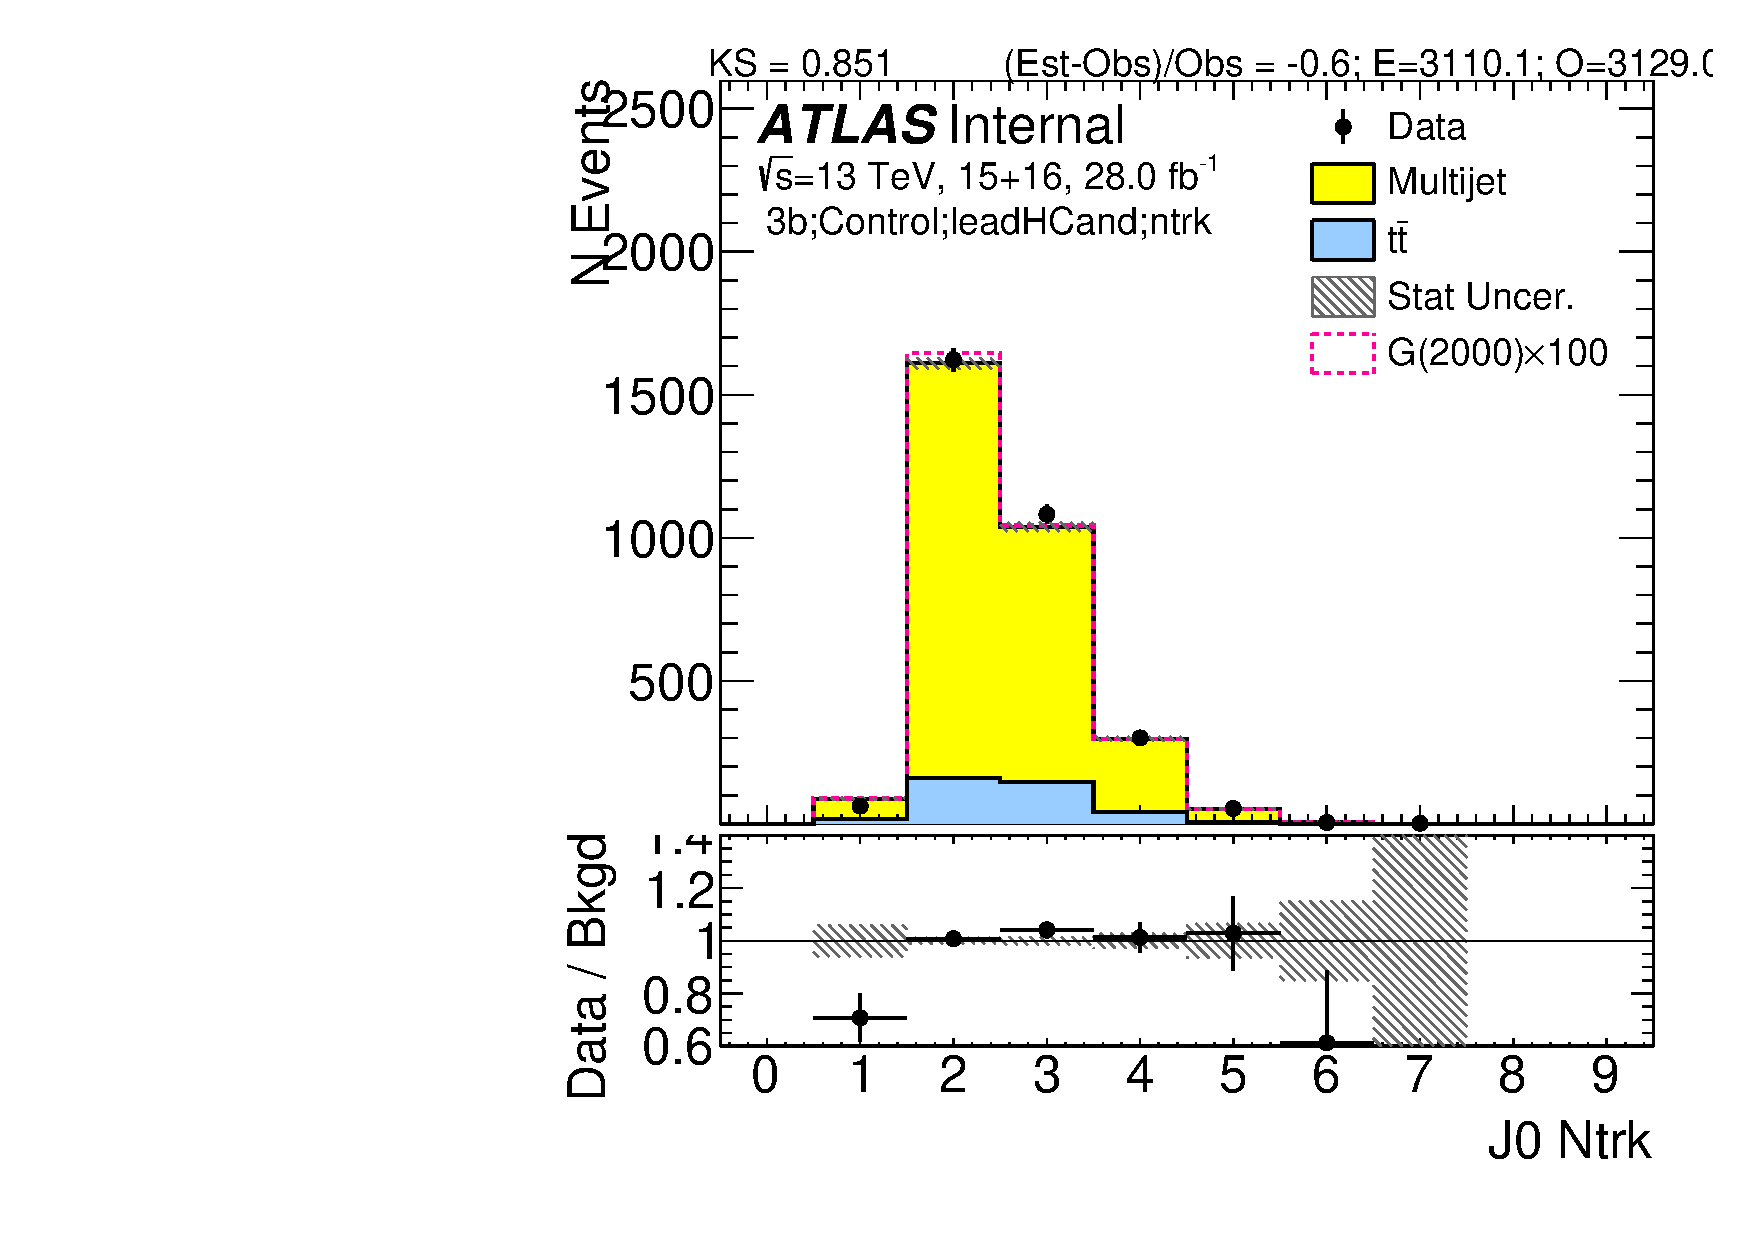
\includegraphics[width=0.45\textwidth,angle=-90]{figures/boosted/Control/b77_ThreeTag_Control_leadHCand_ntrk.pdf}
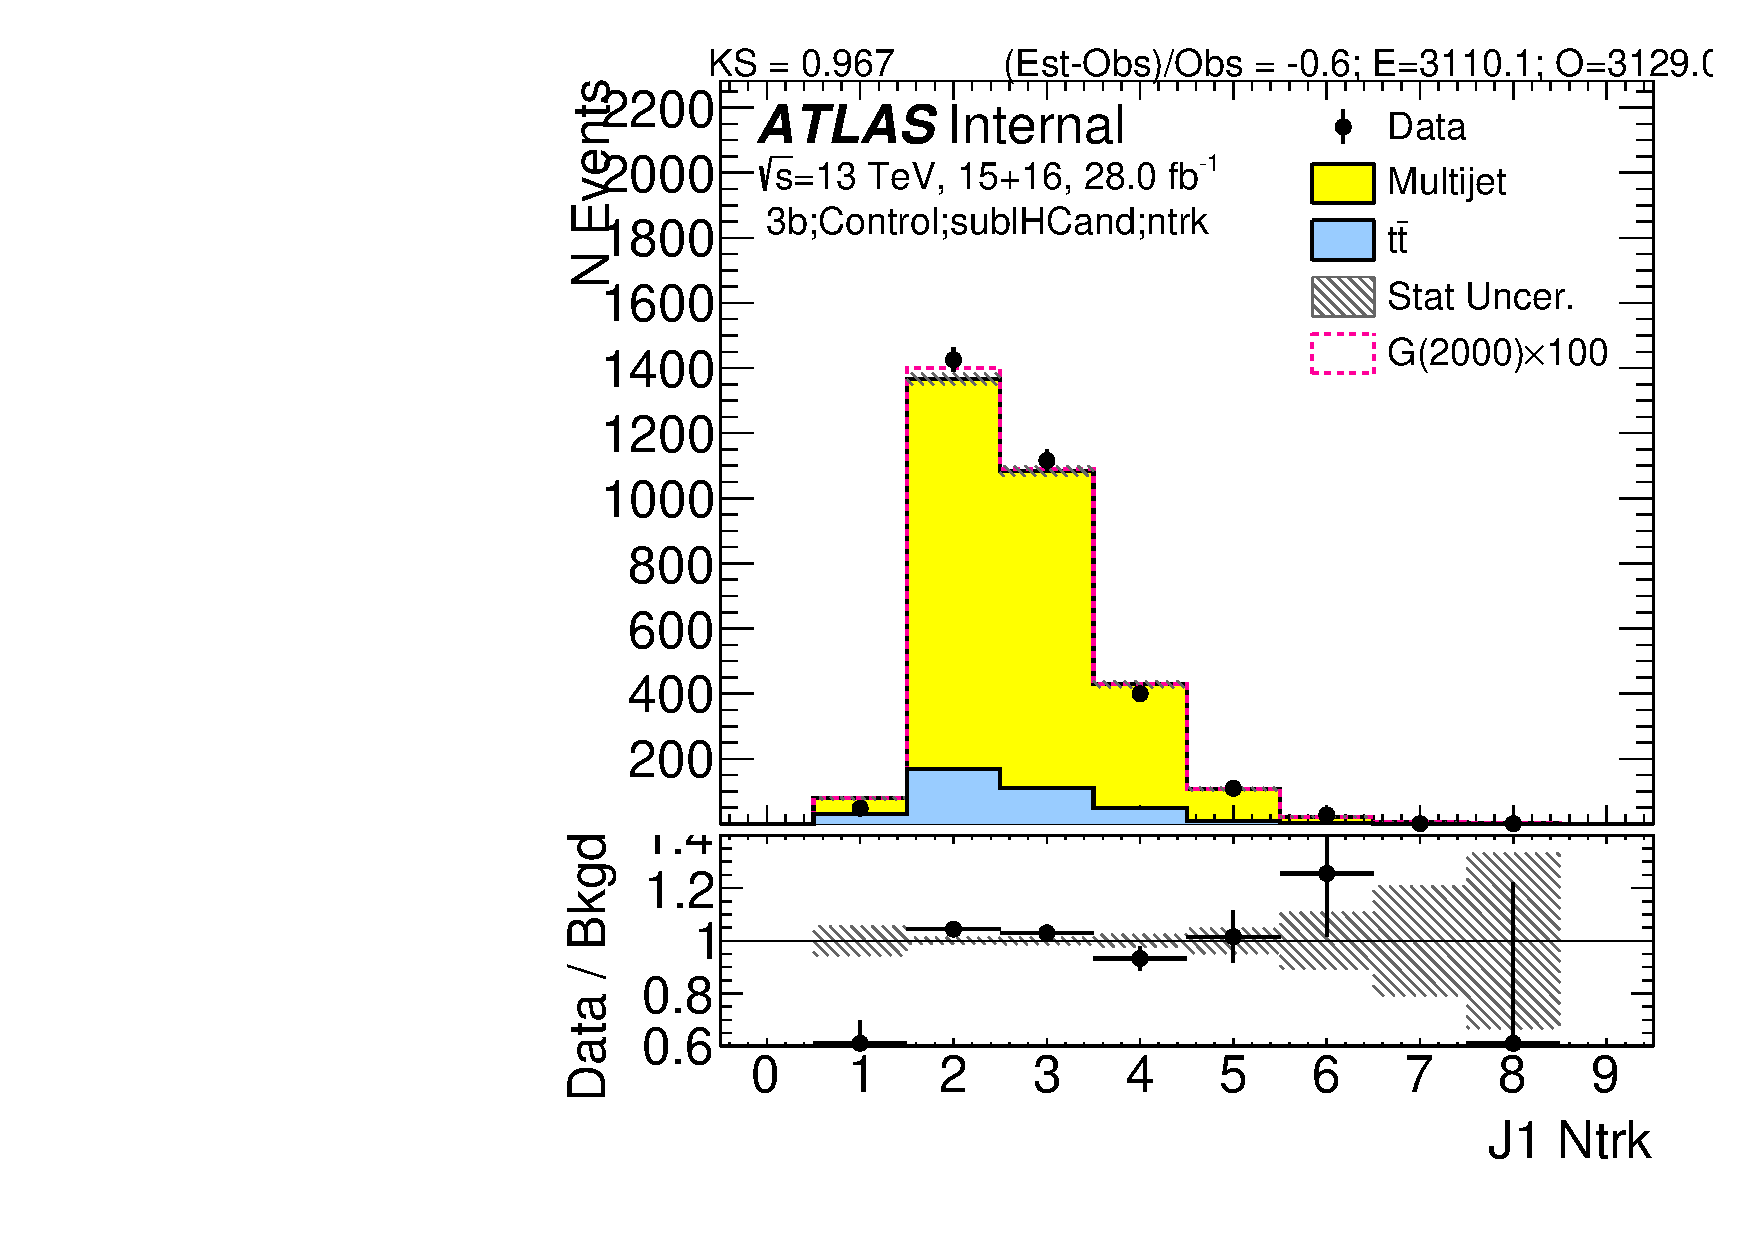
\includegraphics[width=0.45\textwidth,angle=-90]{figures/boosted/Control/b77_ThreeTag_Control_sublHCand_ntrk.pdf}\\
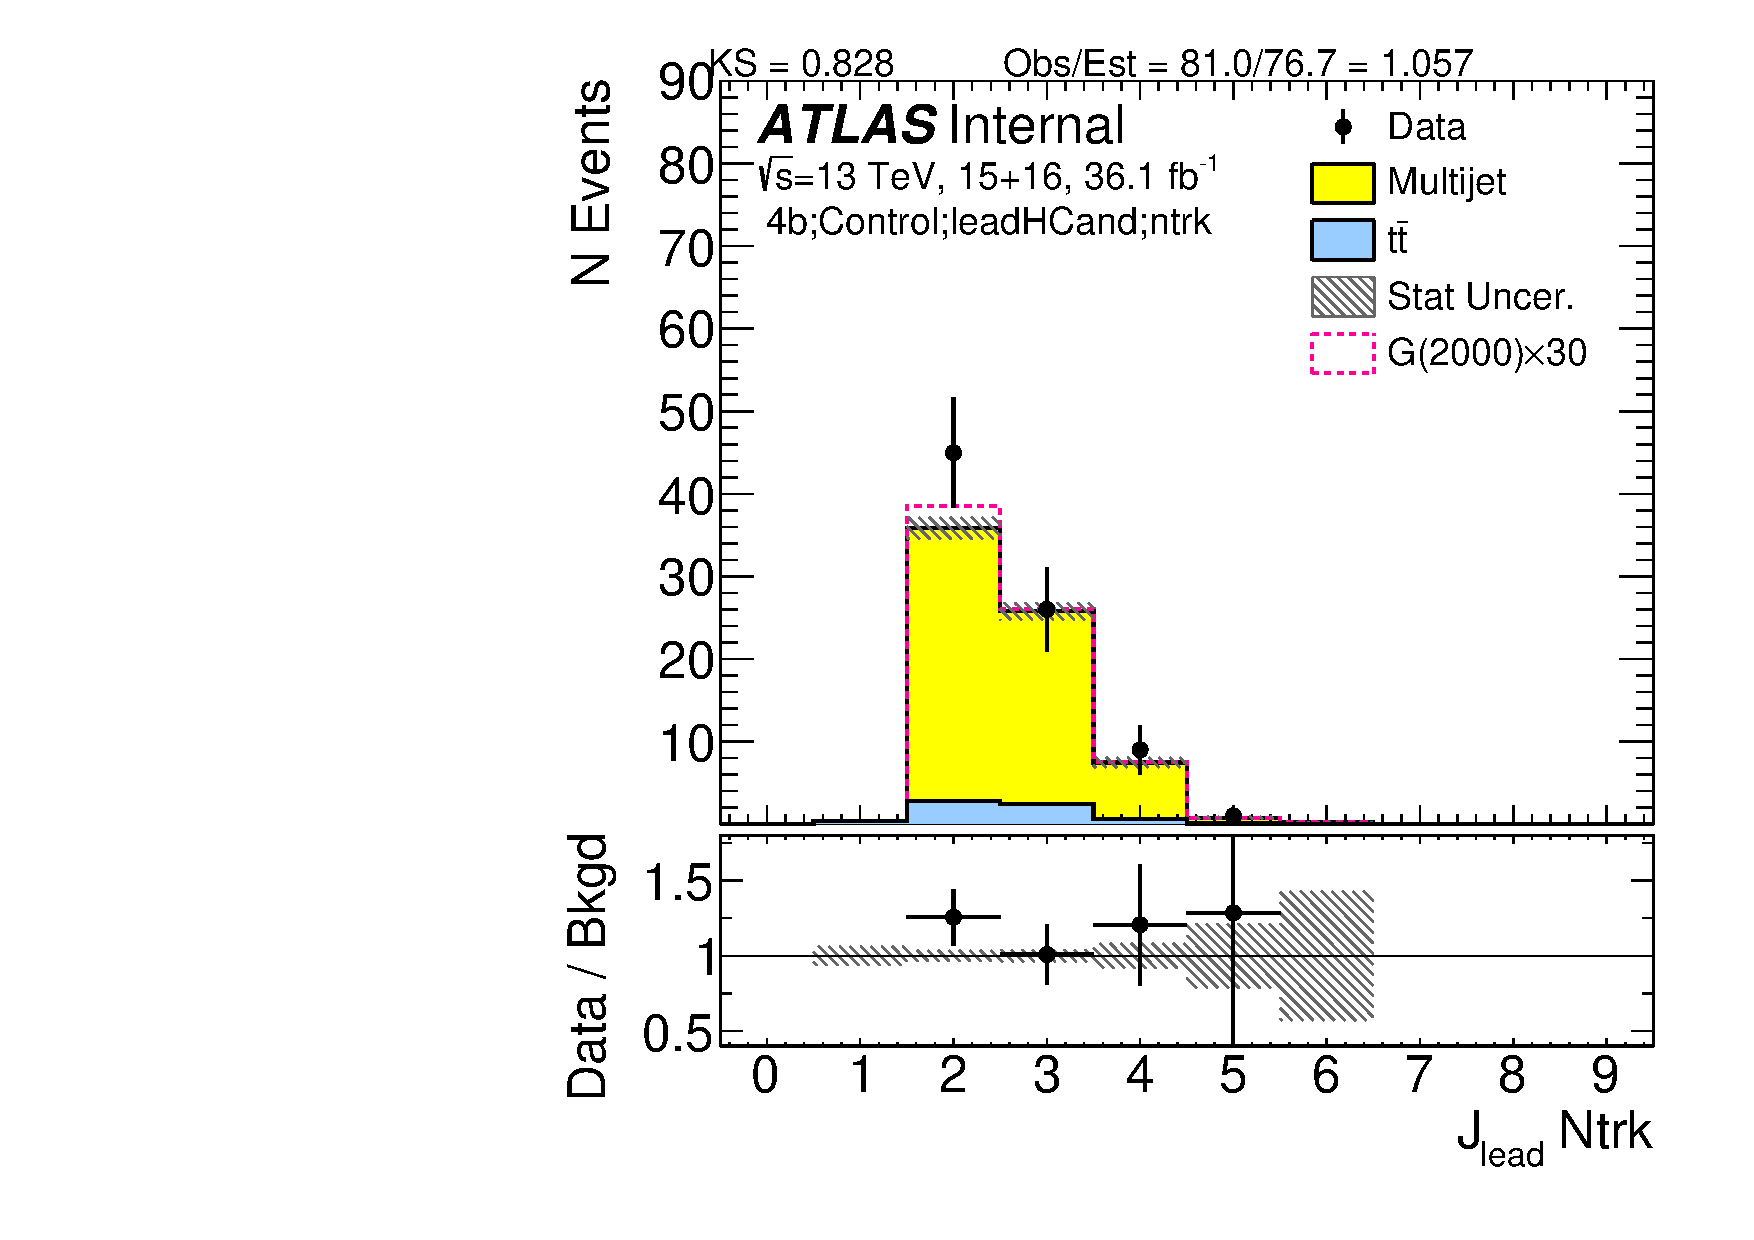
\includegraphics[width=0.45\textwidth,angle=-90]{figures/boosted/Control/b77_FourTag_Control_leadHCand_ntrk.pdf}
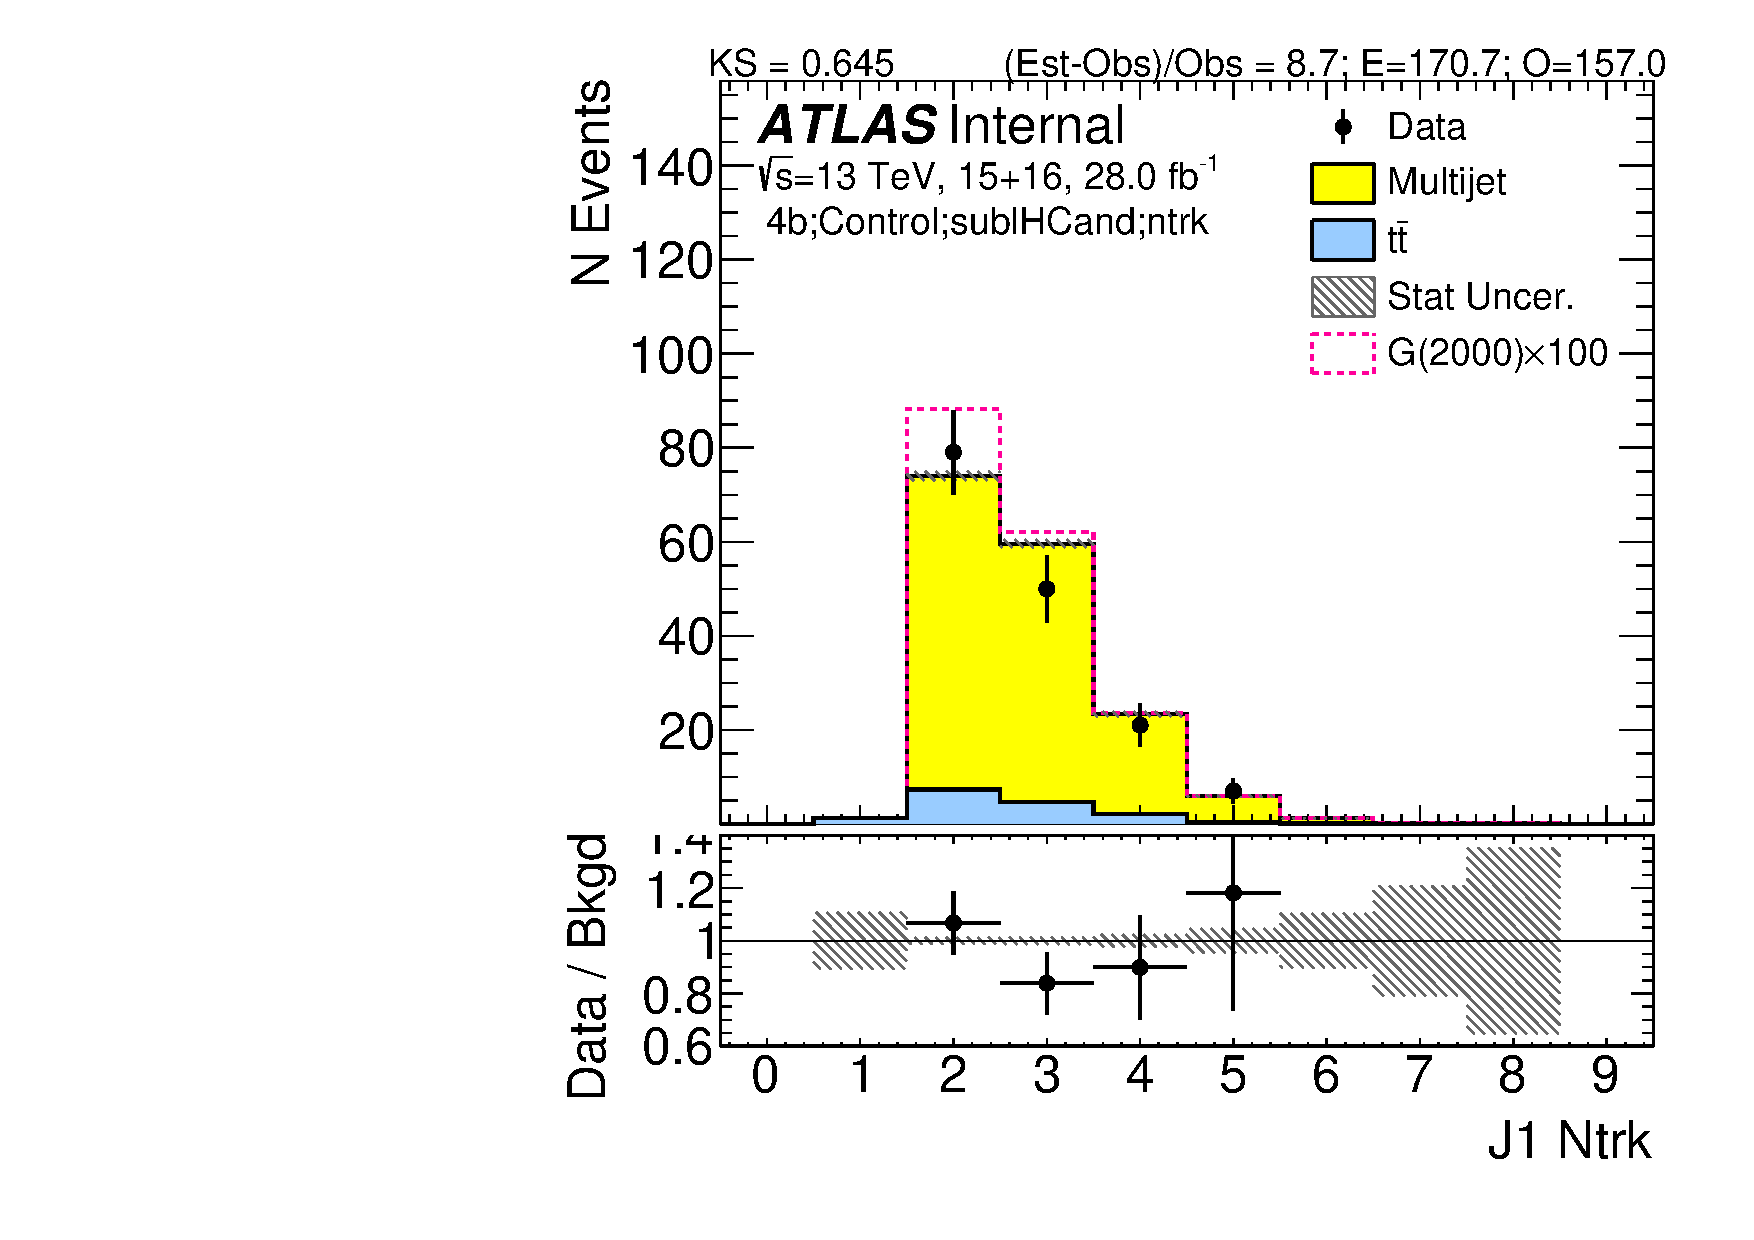
\includegraphics[width=0.45\textwidth,angle=-90]{figures/boosted/Control/b77_FourTag_Control_sublHCand_ntrk.pdf}
  \caption{Number of trackjets in the leading (left) and subleading (right) large-$R$ jet in the Control region for 2bs (top), 3b (middle) and 4b (bottom).}
  \label{fig:boosted-ntrk-Control}
\end{center}
\end{figure*}

\begin{figure*}[htbp!]
\begin{center}
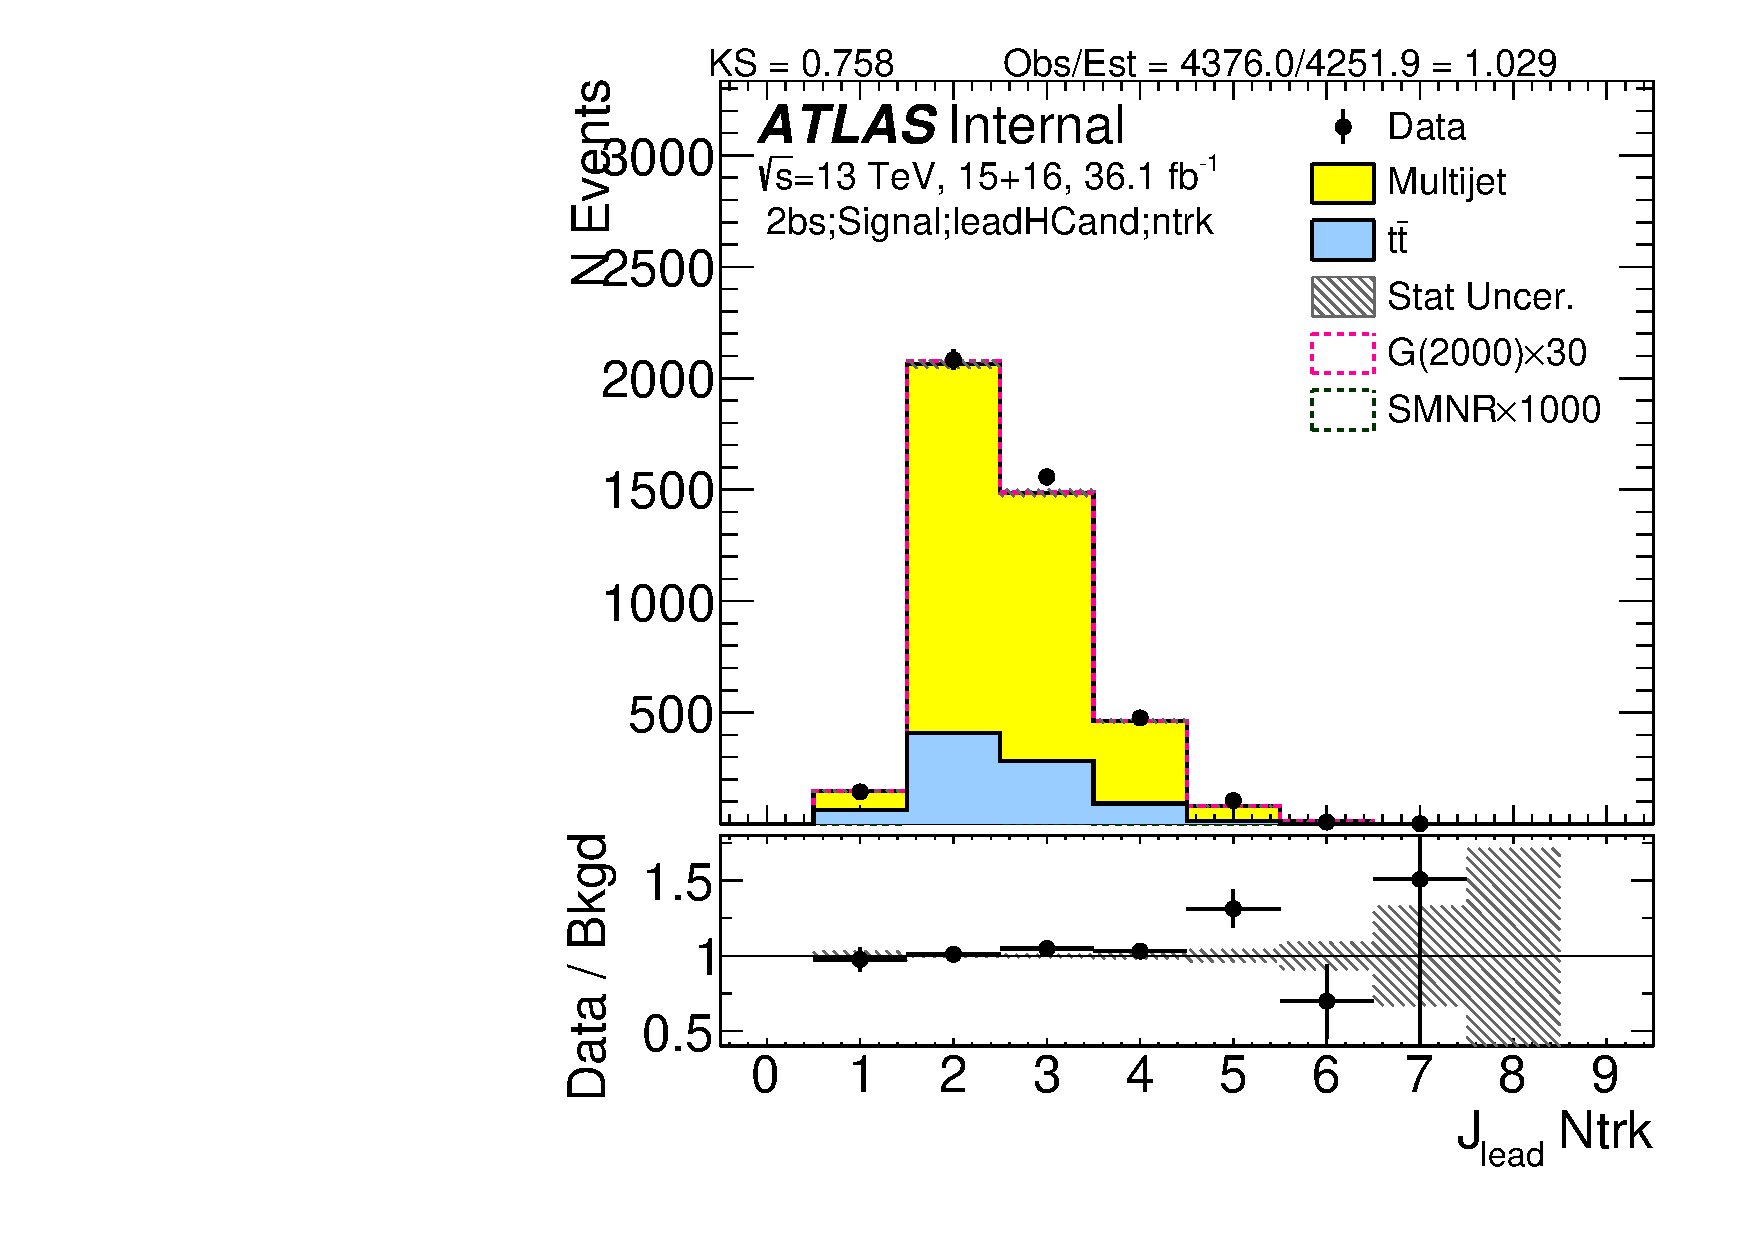
\includegraphics[width=0.45\textwidth,angle=-90]{figures/boosted/Signal/b77_TwoTag_split_Signal_leadHCand_ntrk.pdf}
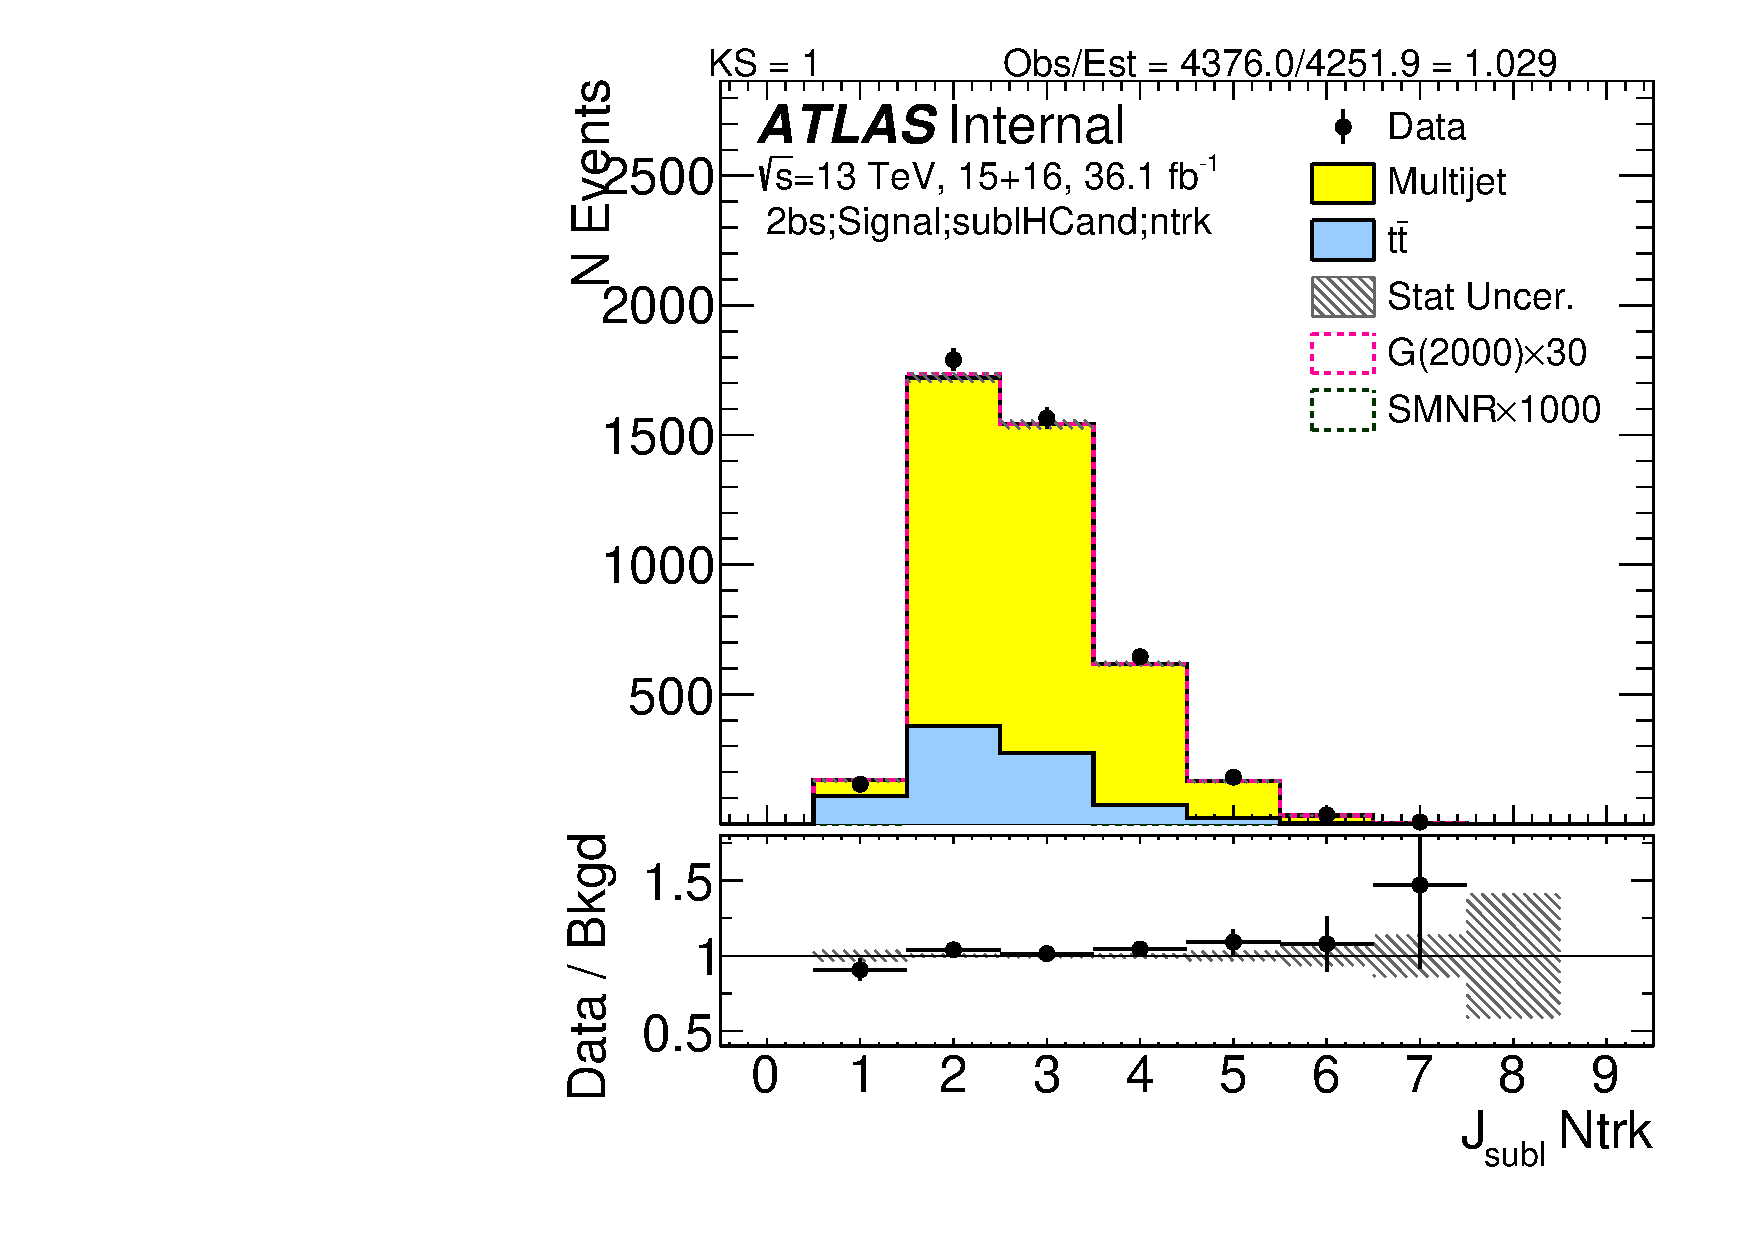
\includegraphics[width=0.45\textwidth,angle=-90]{figures/boosted/Signal/b77_TwoTag_split_Signal_sublHCand_ntrk.pdf}\\
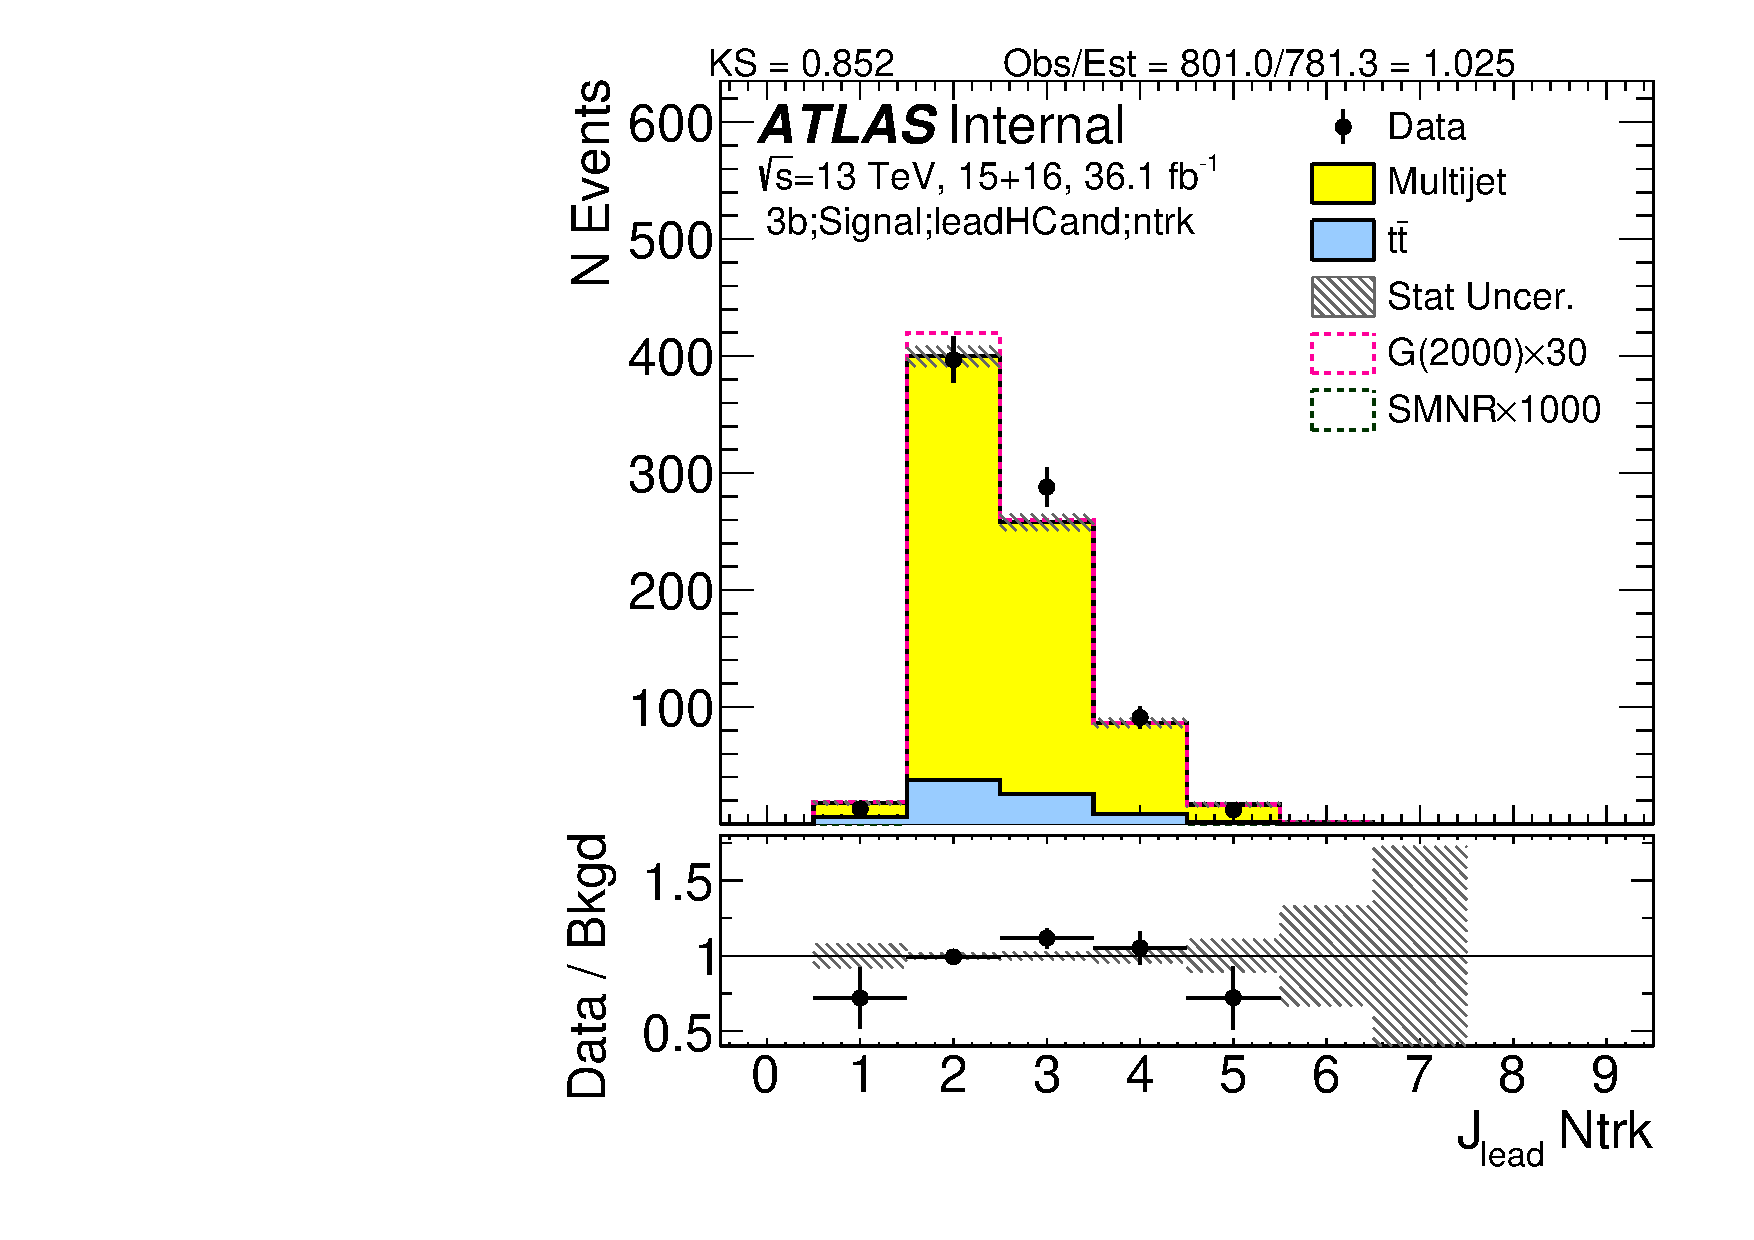
\includegraphics[width=0.45\textwidth,angle=-90]{figures/boosted/Signal/b77_ThreeTag_Signal_leadHCand_ntrk.pdf}
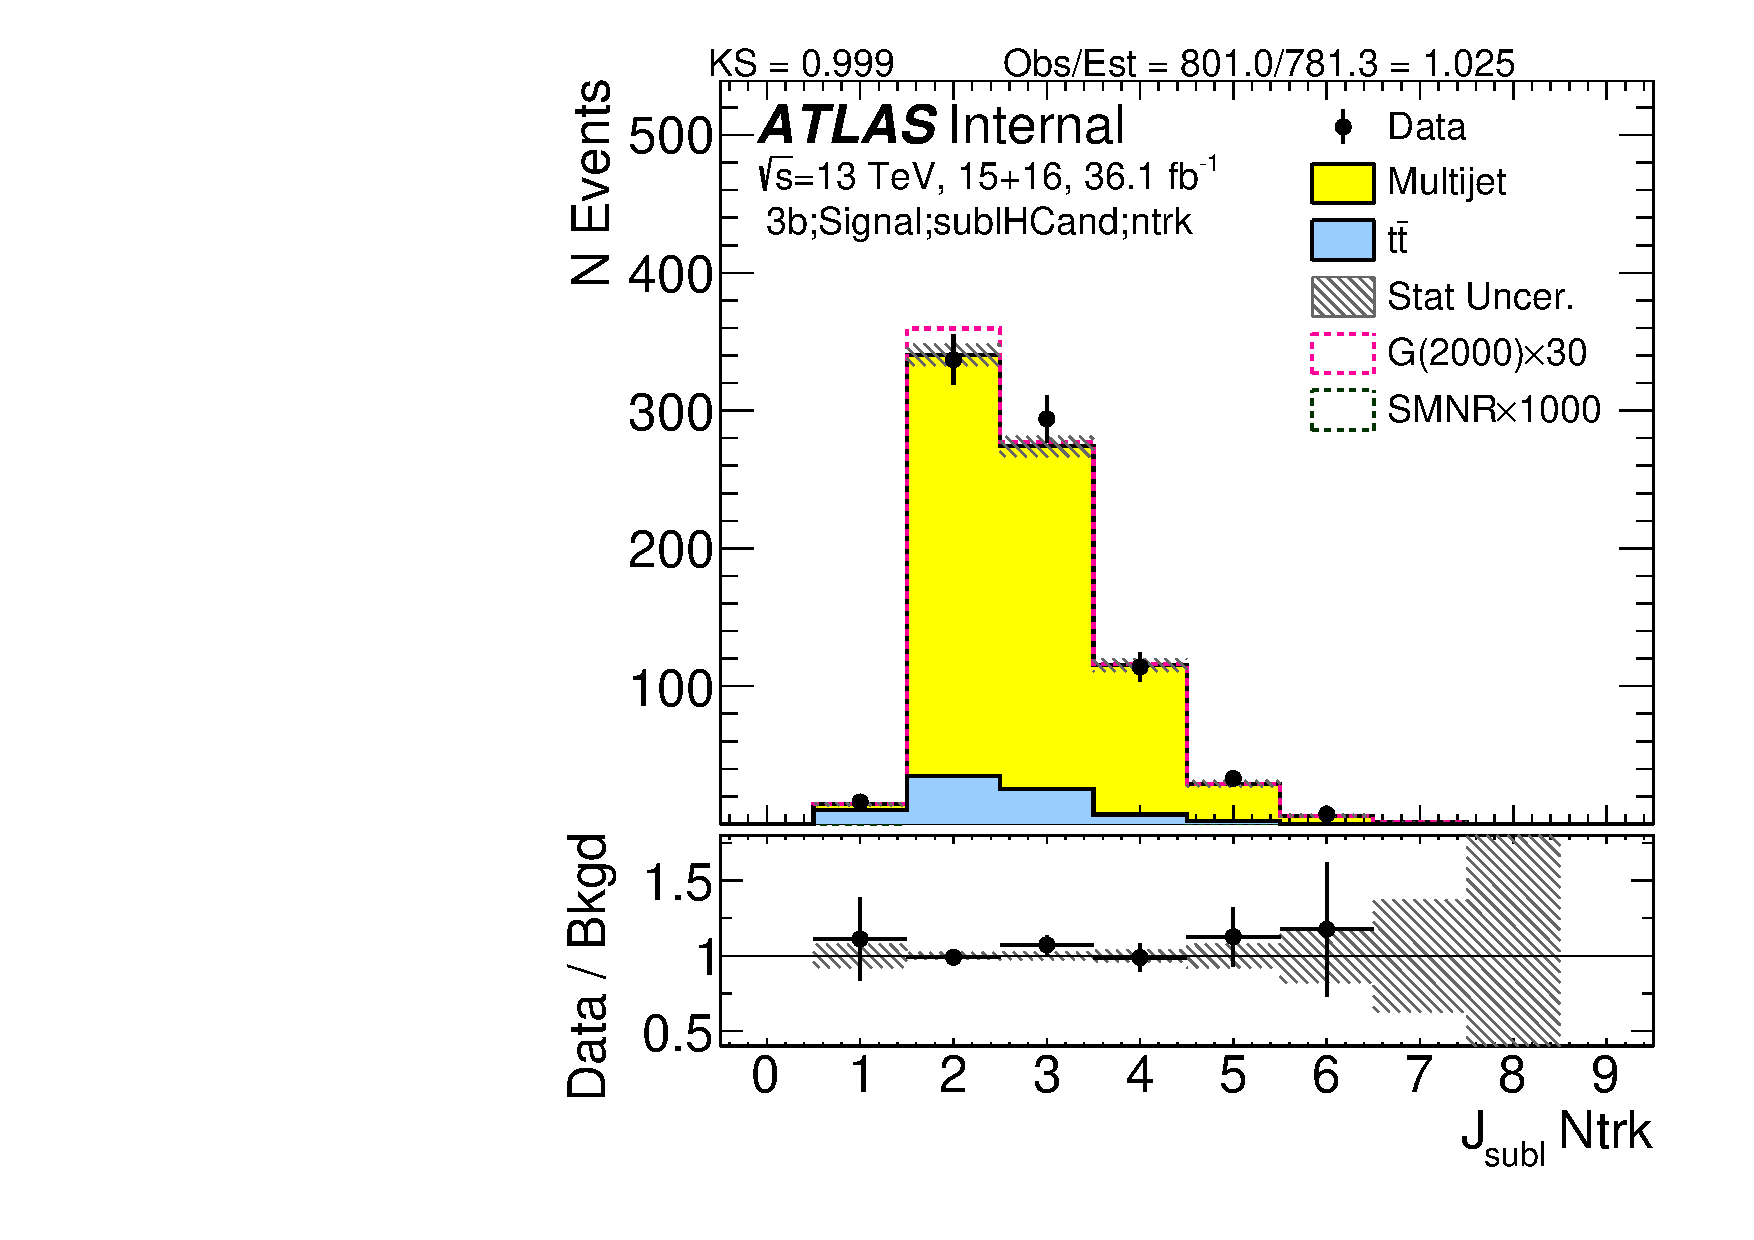
\includegraphics[width=0.45\textwidth,angle=-90]{figures/boosted/Signal/b77_ThreeTag_Signal_sublHCand_ntrk.pdf}\\
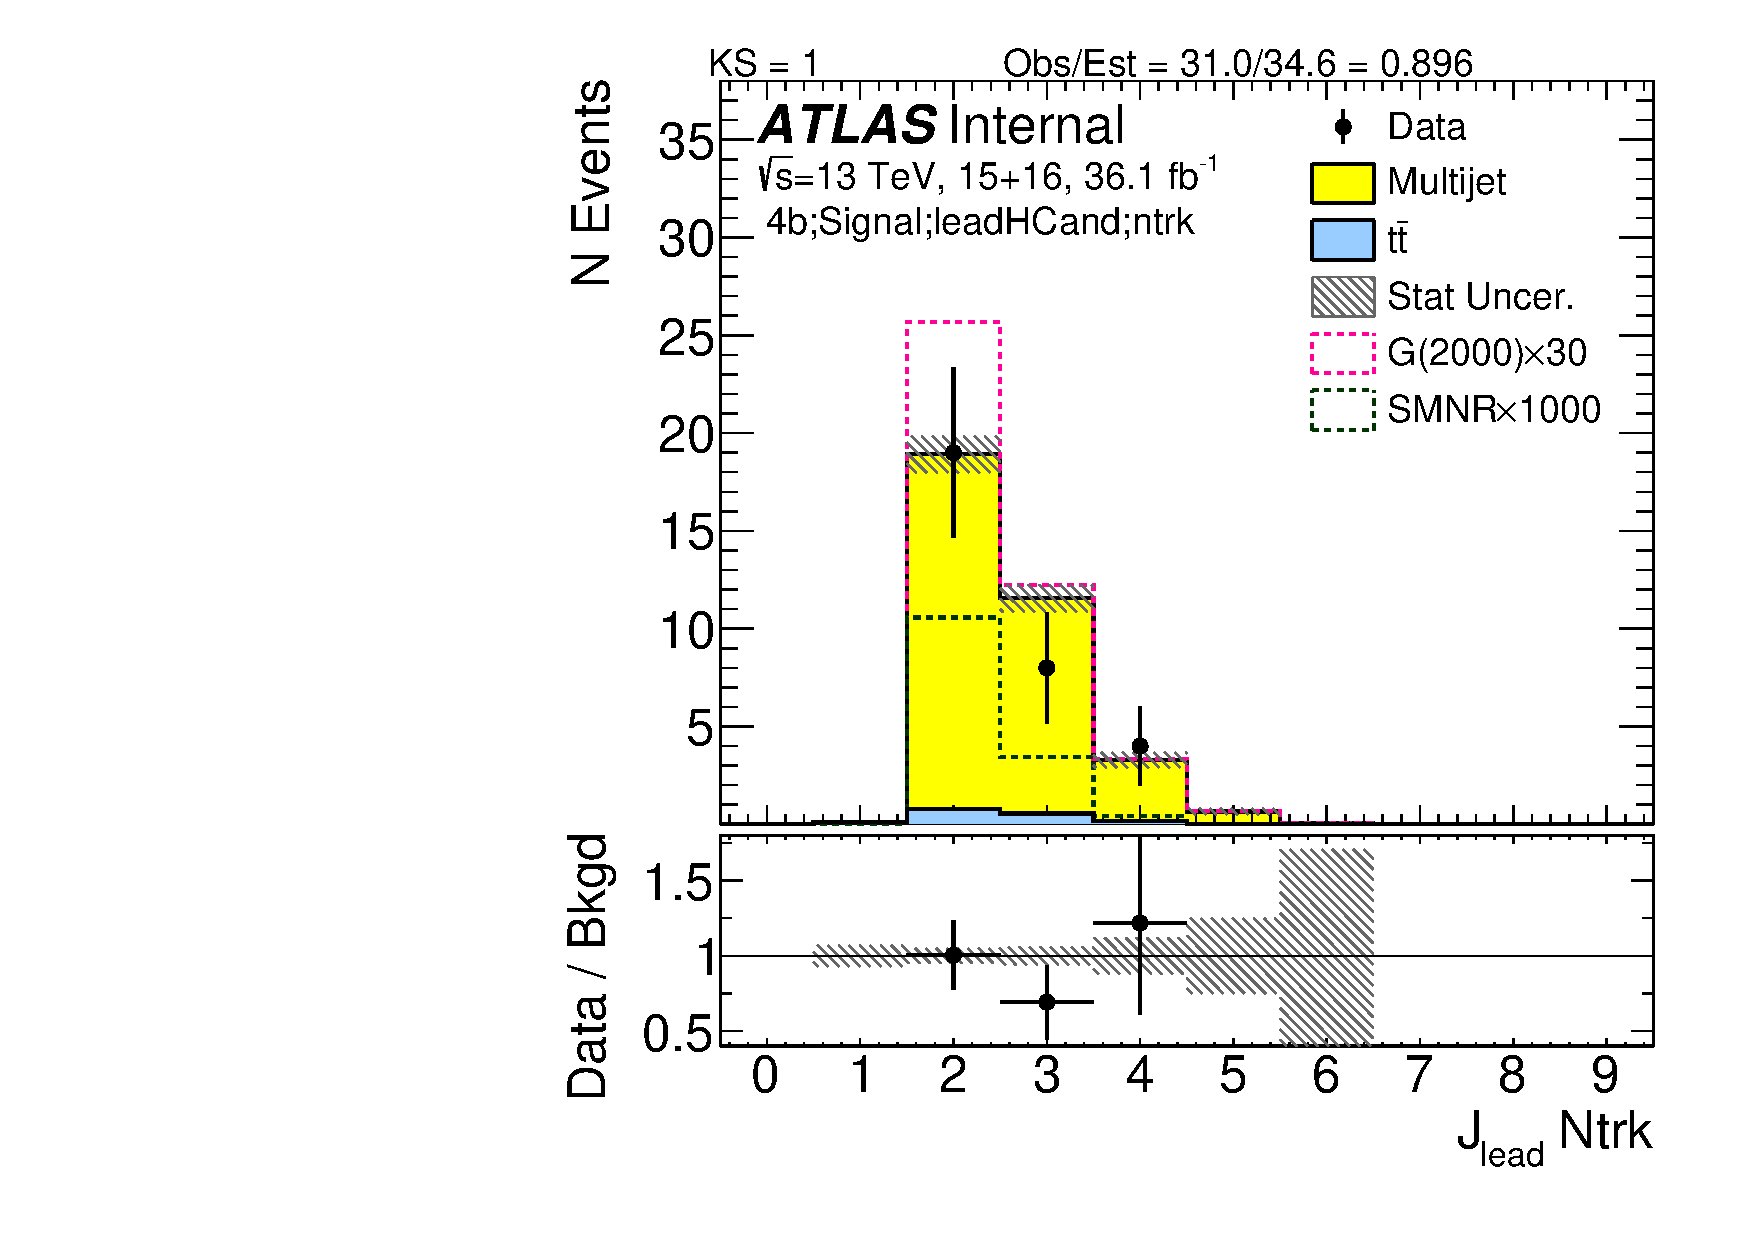
\includegraphics[width=0.45\textwidth,angle=-90]{figures/boosted/Signal/b77_FourTag_Signal_leadHCand_ntrk.pdf}
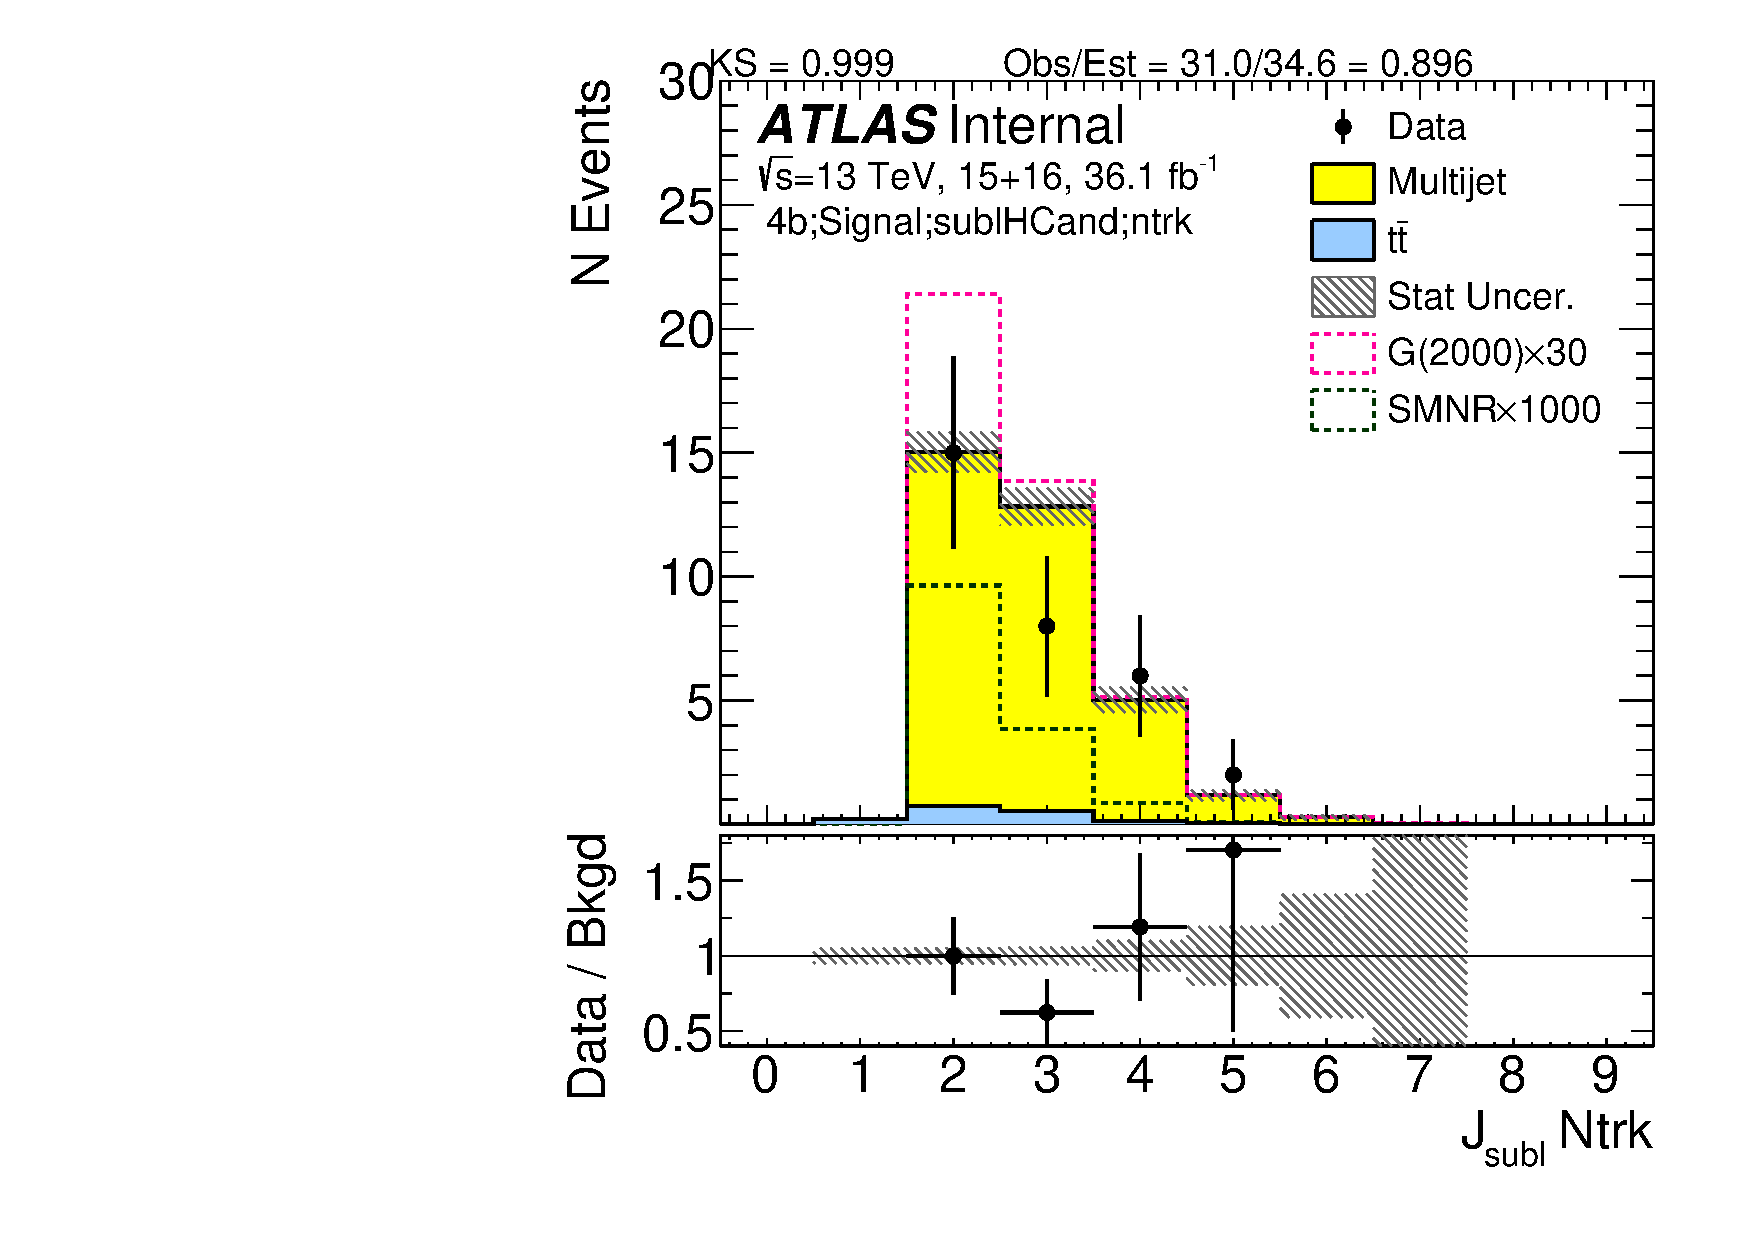
\includegraphics[width=0.45\textwidth,angle=-90]{figures/boosted/Signal/b77_FourTag_Signal_sublHCand_ntrk.pdf}
  \caption{Number of trackjets in the leading (left) and subleading (right) large-$R$ jet in the Signal region for 2bs (top), 3b (middle) and 4b (bottom).}
  \label{fig:boosted-ntrk-Signal}
\end{center}
\end{figure*}